\chapter{典型应用观测与画像分析}\label{chap:profiling}

% 数据中心软件环境的复杂性为任务调度的设计带来了巨大挑战,首先,单一服务器上运行了资源使用差异性大而数量多的应用,应用之间存在隐含的资源竞争,其次,网络服务类型应用负载存在波动,不同负载下应用的特征也存在差异。

% 针对如上挑战,本章首先分析了数据中心软件环境的组成,通过选取典型应用的方式提炼重要的监测对象,并结合与云厂商的合作经验选取了7种典型应用作为画像目标。

% 虚拟机时云场景中主要的运行时环境,为解决虚拟机所引入的黑盒性能监测的问题,本章中设计了一套面向虚拟机的可观测性系统,通过广泛的性能指标采集来解决虚拟机的性能监测问题。

% 最后,本章设计了有干扰实验与无干扰实验,分析不同应用在资源使用倾向与敏感度上的特点与差异。

为解决数据中心的软件环境复杂性带来的挑战,本章围绕数据中心典型应用展开监测画像,研究应用的资源使用倾向即资源敏感度。首先,结合对数据中心软件栈分析以及与云厂商的合作经验,选择了一批典型应用,并采用云环境中广泛使用的虚拟机作为应用运行环境。随后,围绕虚拟机设计实现了一套黑盒可观测性系统,从Host、Hypervisor与Guest等多个维度,采集丰富的指标信息。最后,在可观测性系统的基础之上展开对典型应用的资源倾向与敏感度实验,并给出画像结论。

\section{云场景典型应用选择}

% 软件环境复杂 -> 应用需求不同 -> 软件架构复杂 -> 存在共性的基础应用 -> 基础应用的性能是整体性能的关键 -> 选取典型应用进行分析


数据中心应用越来越多地采用微服务架构,一些职责单一、功能类似的服务被抽象为公共组件,如数据库、键值存储、消息中间件等。同时随着开源软件社区的不断发展,越来越多的开源公共组件被应用到不同的项目中。公共组件通常在请求的关键路径上提供服务,并在一定程度上影响应用整体性能。本文结合与云厂商的合作经验,选择了一批云场景中的典型公共组件作为主要的画像对象,涵盖了传统数据库、键值存储、消息中间件、媒体处理等领域,具体应用如表~\ref{tab:typical_application}所示。

\begin{table}
    \bicaption{\quad 云场景典型应用}{\quad Typical Applications in Cloud Scenarios}% caption
    \label{tab:typical_application} 
    \footnotesize% fontsize
    \setlength{\tabcolsep}{4pt}% column separation
    \renewcommand{\arraystretch}{1.25}% row space 
    \centering
    \begin{tabular}{lc}
        \hline
        %\multicolumn{num_of_cols_to_merge}{alignment}{contents} \\
        %\cline{i-j}% partial hline from column i to column j
        类型 & 应用\\
        \hline
        SQL & mysql\\
        NoSQL & elasticsearch\\
        Web Server & nginx\\
        K-V Store & redis、memcached\\
        Message Queue & kafka\\
        Media & render\\
        \hline
    \end{tabular}
\end{table}

这些典型应用在用途上及实现上的差异,意味着会使用到不同的资源,并对对调度机制有不同的需求:

\begin{itemize}
    \item \textbf{数据库类型的应用}:如Mysql,传统的关系型数据库提供了完善的数据存储、检索查询及事务管理等功能,实现中原始数据通常保存在磁盘上,在进行大量数据查询时,不仅会使用到较多的CPU资源,同时也会占用相当的IO资源,因此需要调度器保障其CPU资源,并避免IO上的干扰。
    \item \textbf{键值存储类应用}:如Redis、Memcached,通常作为信息缓存服务,提供快速的数据存储与查询,由于数据存储在内存中,因此对内存资源存在较高要求,对调度的需求主要体现在两方面,一方面需要足够的内存资源,另一方面则需要避免在内存带宽上的干扰。
    \item \textbf{网络服务类型应用}:如Nginx,网络页面通常都具有交互属性,而延迟会极大影响用户的使用体验,因此这类应用要求调度能够在网络请求到达时,及时的为网络服务分配CPU,以尽早地对用户请求进行处理。
    \item \textbf{媒体处理应用}:通常是离线应用,运行时一方面会占用IO资源,用来读写媒体素材,另一方面会占用CPU资源,来进行编解码操作,这类应用需要调度分配足够长的时间片,同时希望能减少上下文切换,以便更好地利用局部性来加快执行速度。
\end{itemize}

应用的运行依赖一定的软件环境。云场景中为达到足够的隔离性,避免多租户间的相互影响,通常会采用沙箱环境隔离不同的应用。本文结合与云厂商的合作经验,选择云厂商使用较广泛的KVM虚拟机作为应用的沙箱环境。

\section{观测系统设计与指标收集}

\subsection{面向虚拟机的多维指标采集设计}

% 分解虚拟机: Host侧 -> Hypervisor侧 -> 应用侧
% 分解采集系统:
% - 采集侧
% - 查询、存储、分析侧

KVM虚拟机相对黑盒的运行环境为应用性能的监测带来了挑战。而为解决虚拟机场景下的应用性能分析问题,本文通过从不同维度采集丰富的指标信息,提供更全面、深入的观测,来推断应用的性能。

本文从如图~\ref{fig:vm_arch}所示的Host、Hypervisor、Guest三个维度来设计指标采集方式。

\begin{figure}[!htbp]
    \centering
    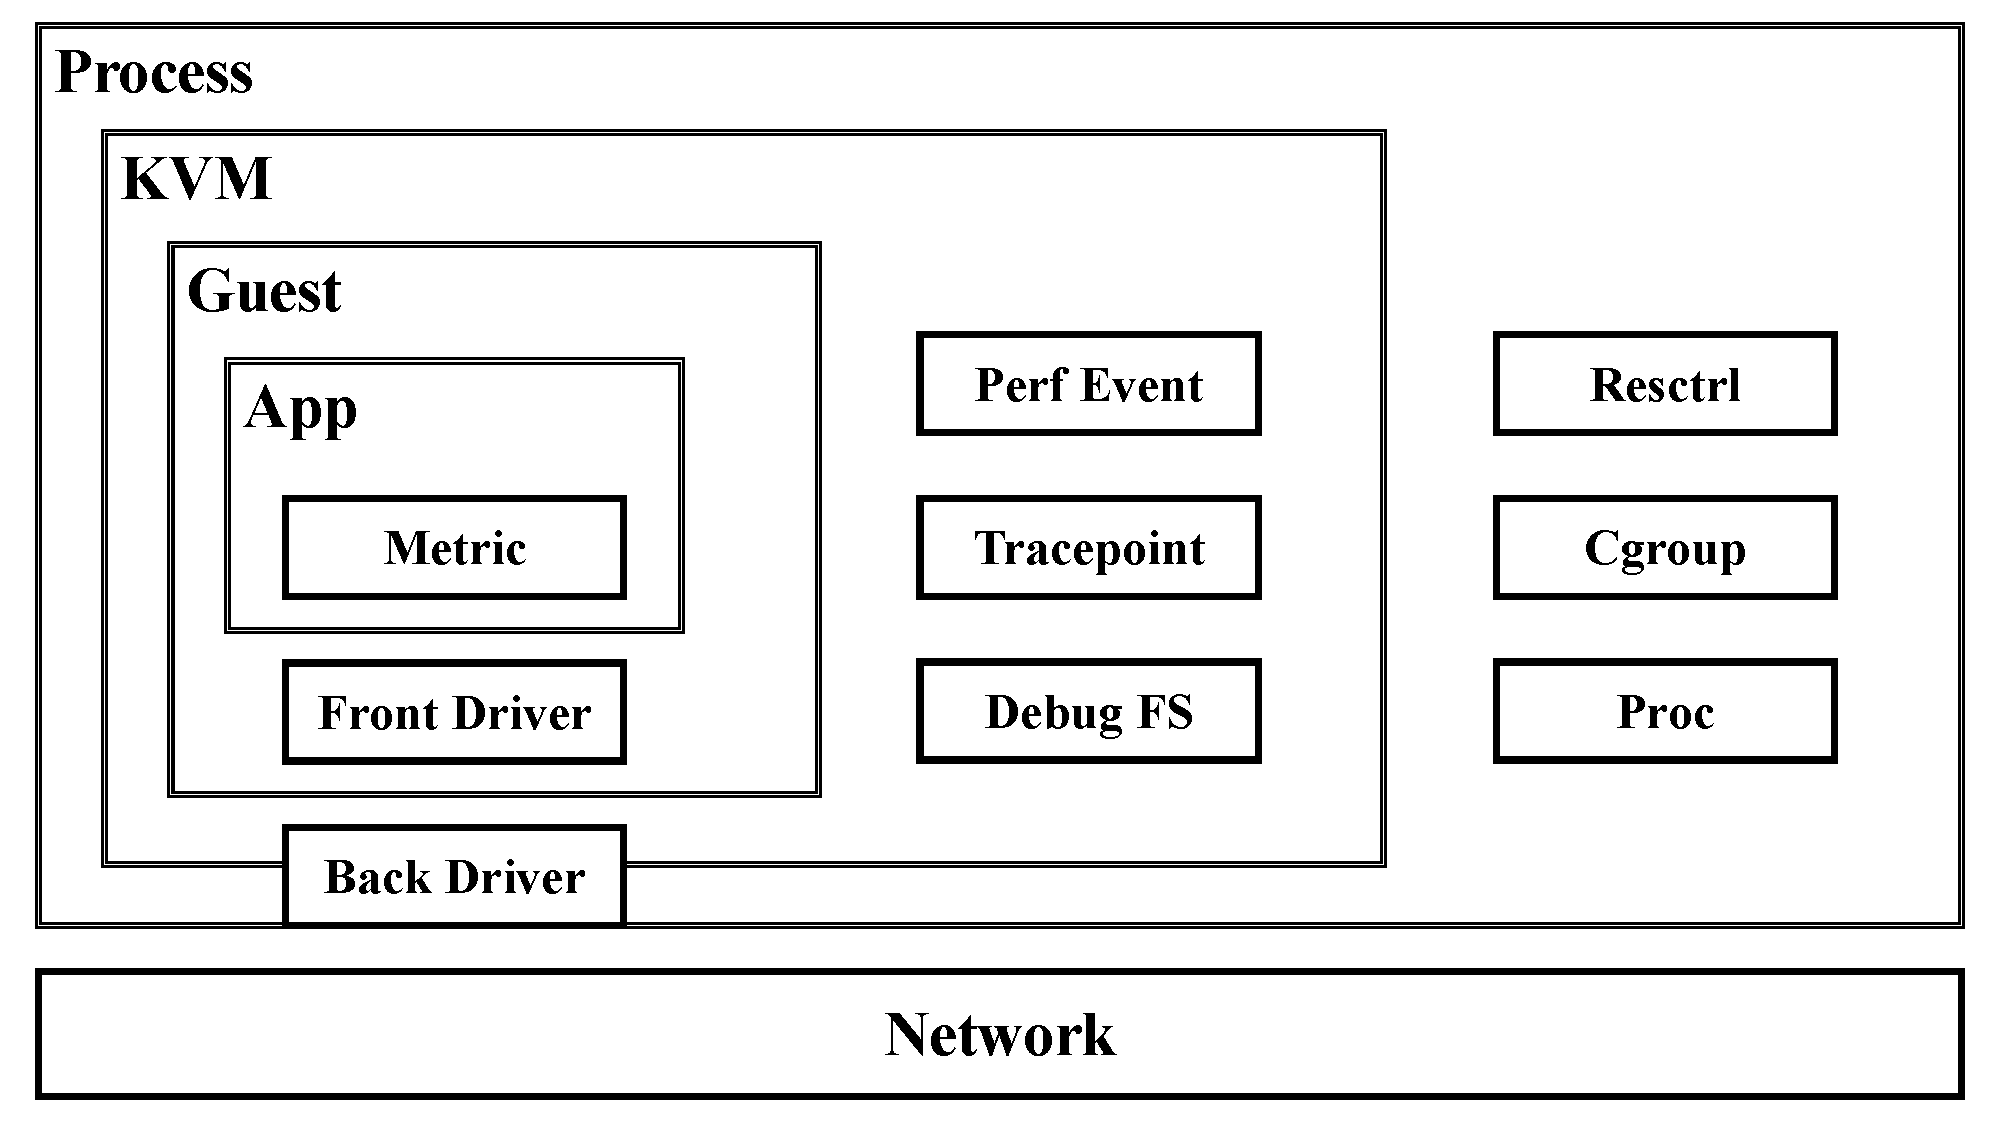
\includegraphics[width=0.6\textwidth]{vm_arch}
    \bicaption{\quad 虚拟机多维度指标采集}{\quad Multi-dimensional metrics from virtual machines}
    \label{fig:vm_arch}
\end{figure}

在Host维度,KVM虚拟机本身由多个进程组成,因此可以利用Host内核提供的进程观测接口来获取虚拟机的指标信息。如通过“/proc”内核文件系统来获取进程内核资源使用统计信息,或者利用cgroup来获取进程的CPU时间记账信息等。在Hypervisor维度,虚拟机使用的虚拟硬件设备如vCPU、Block设备、Network设备等由Hypervisor提供,因此可以利用KVM内核模块提供的虚拟设备观测接口来获取相关信息。如在KVM模块的Debug内核文件系统中,就提供了丰富的vCPU设备运行信息,包括IO、挂起、中断等vCPU陷出统计,以及模拟MMU缓存缺失统计等。在Guest维度,一方面可以从Guest内核侧获取应用的资源使用信息,另一方面对于C-S类型的网络服务应用,则能够利用Overlay网络层来对请求的延时、吞吐进行观测。同时,大部分开源的应用都提供的完善的观测接口,能够提供更加准确的性能指标。

Linux内核提供的观测接口有限,而为提供更丰富的内核观测数据,本文基于eBPF设计了多种内核监测机制。Linux中进程对硬件资源的使用通常需要通过系统调用完成,如通过Send、Recv等系统调用来使用网络资源、通过Read、Write等系统来使用IO资源。常用的系统调用观测工具为strace,但在云场景中使用strace并不方便且不够灵活。而本文使用eBPF在系统调用分发处进行插桩,并能够捕获系统调用的参数与返回结构,从而定制更灵活的信息统计机制。不同于进程,虚拟机使用硬件资源的方式更为特殊。以网络资源为例,早期虚拟机的实现中需要两次陷出到用户态Qemu程序再进行网络设备的模拟,这种方式严重影响了虚拟机的网络性能。而为提升虚拟机使用网络资源的性能,一方面在Guest侧引入了virtio半虚拟化驱动,另一方面在宿主机上引入了vHost net网络设备。如图~\ref{fig:vhost_net}所示,vHost net作为一种内核态实现的模拟网络设备后端,在虚拟机首次陷出后就直接进入vHost Net模块,并最终由Worker内核线程完成网络包的处理。通过eBPF在Worker线程函数上的插桩,就能够观测虚拟机模拟网络设备后端的性能。

\begin{figure}[!htbp]
    \centering
    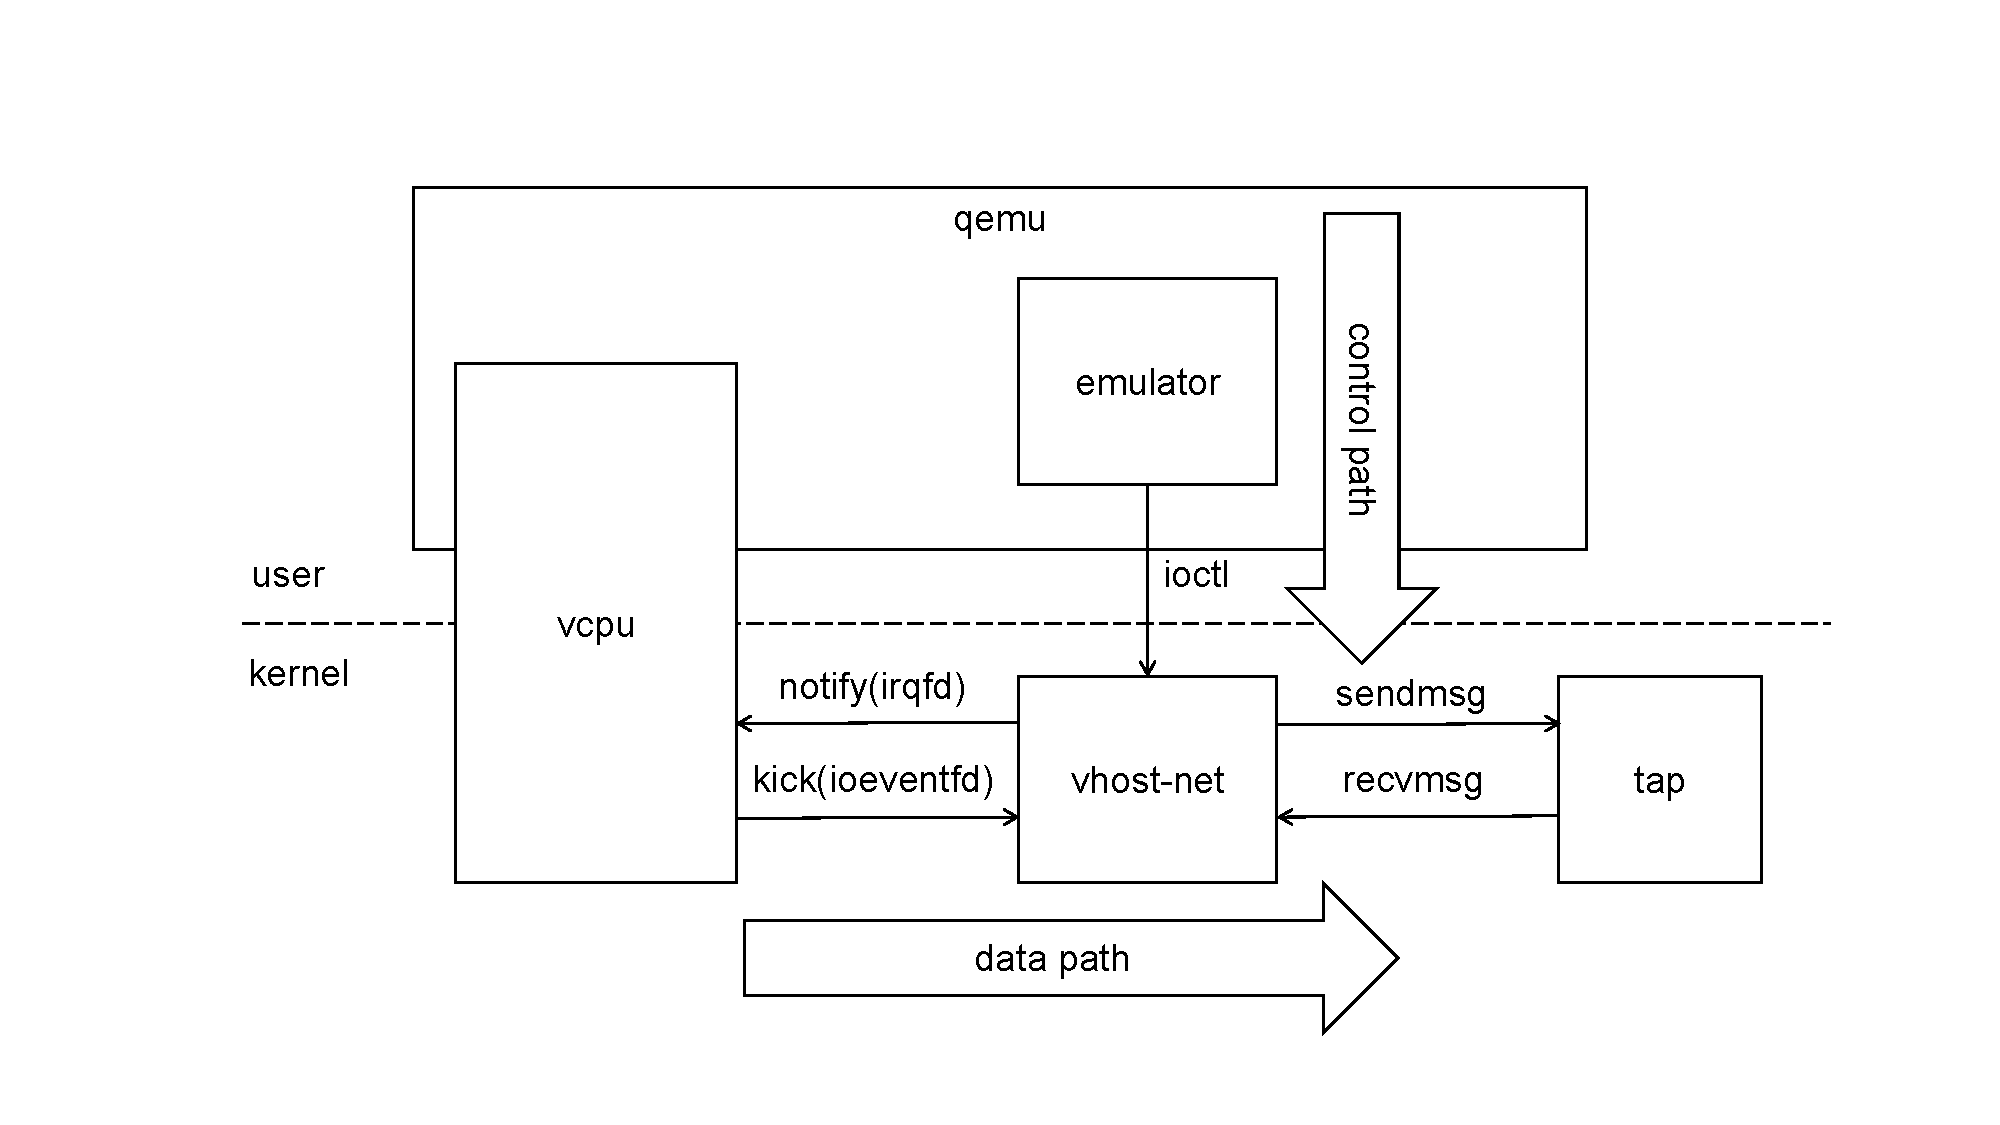
\includegraphics[width=0.6\textwidth]{vhost_net}
    \bicaption{\quad vHost Net模拟网络设备后端}{\quad vHost Net Simulate network device backend}
    \label{fig:vhost_net}
\end{figure}

综合以上分析,本文设计了一种实时指标采集分析系统,从Host、Hypervisor、Guest三个维度以虚拟机为粒度进行指标采集,并提供指标的存储、查询与分析服务。观测系统占中定义了Observer与Observed两种角色,并采用统一的指标编码。其中,Observed角色对外暴漏指标采集接口,Observer角色则周期性地轮询以获取指标数据。Observer角色还需要将获取到的指标进行存储,并提供基本的查询服务。系统中可以有多个Observer角色来分摊采集压力,节点也可以按需要同时承担Observer与Observed角色。

\subsection{实时可观测性系统实现}

% Observer实现
% - Prometheus、Grafana、Collector Utils
% Observed实现
% - Exporter的实现细节
%   - Ebpf Exporter
%       - Syscall 追踪
%       - vHost Net 追踪

\begin{figure}[!htbp]
    \centering
    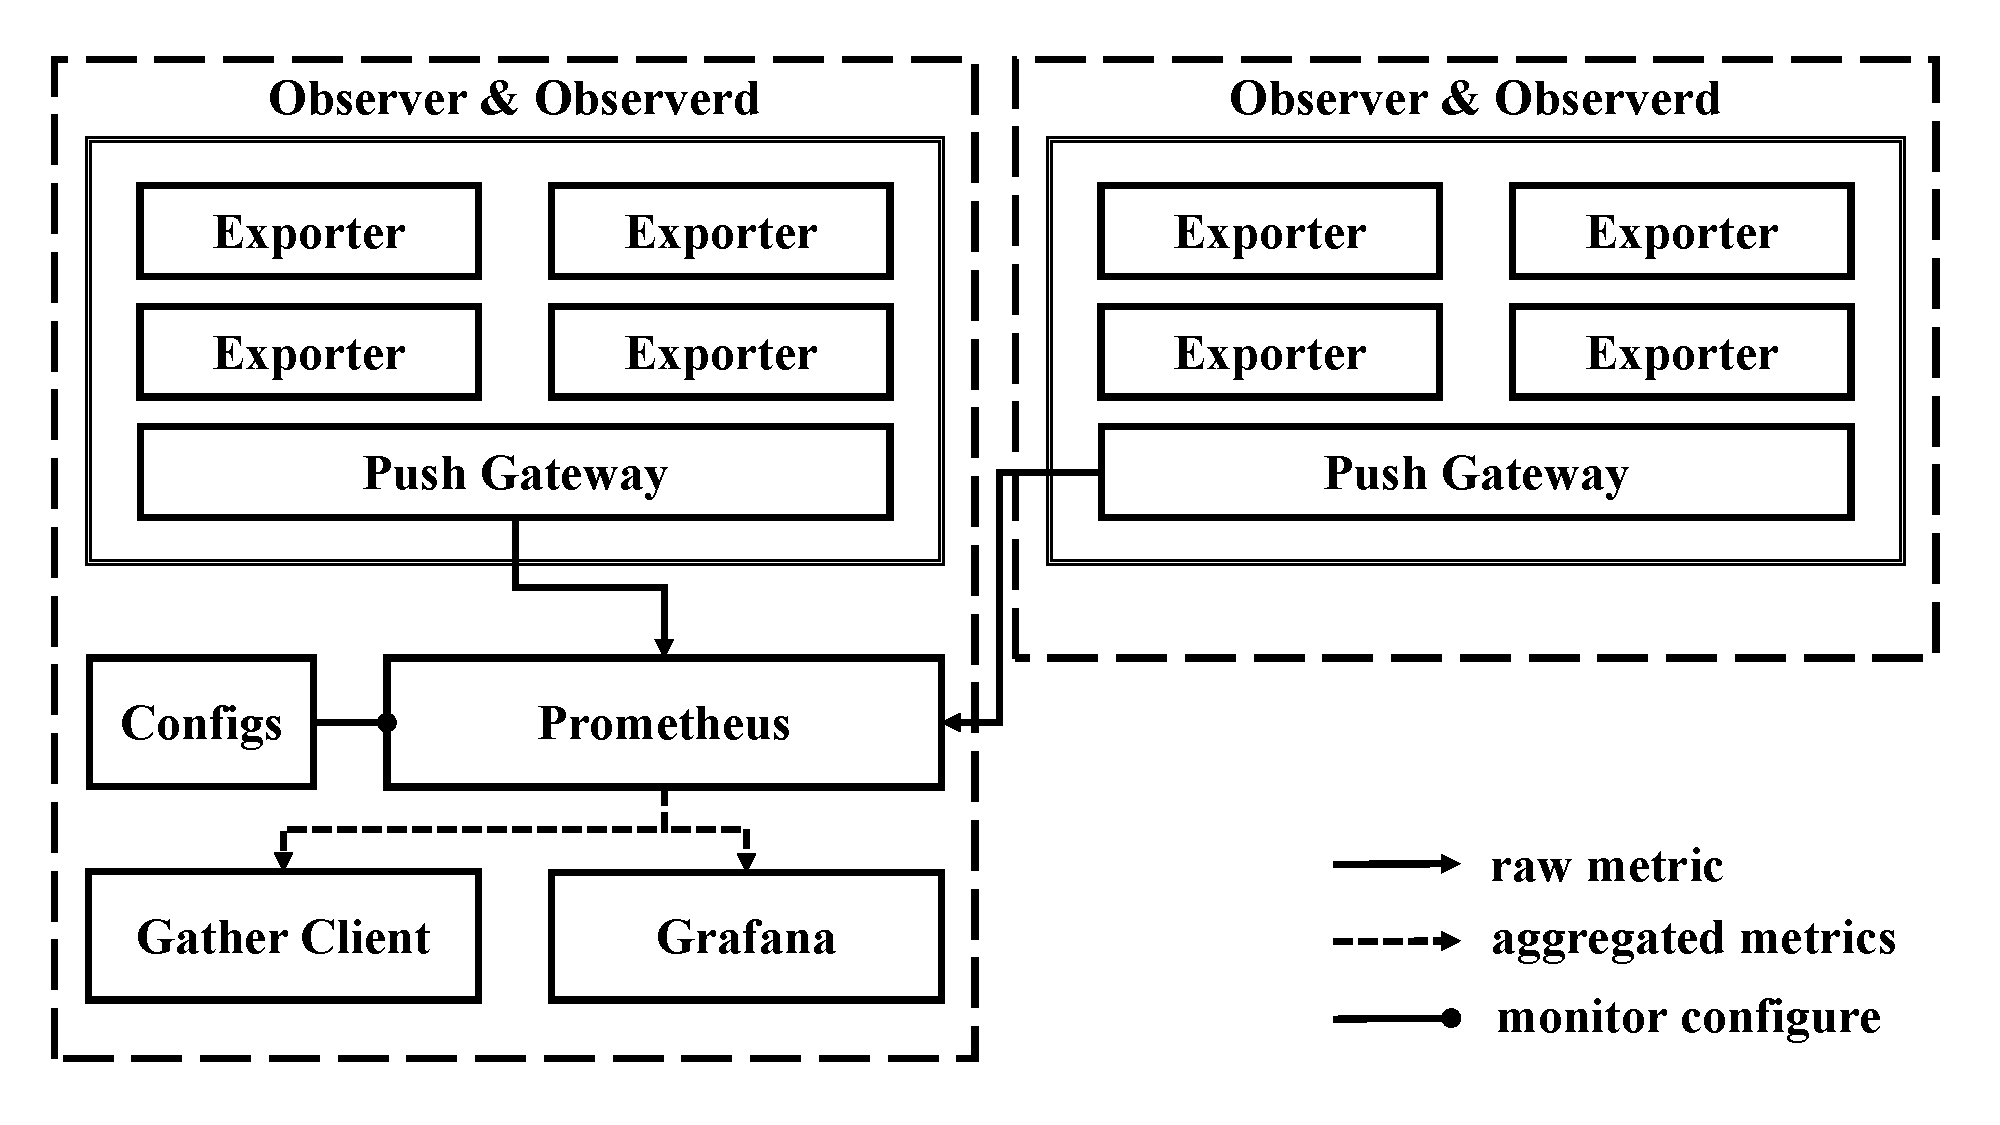
\includegraphics[width=0.75\textwidth]{monitor_arch}
    \bicaption{\quad 采集系统架构}{\quad Metric Collection System Architecture}
    \label{fig:monitor_arch}
\end{figure}

本文结合云原生的实践经验,基于Prometheus\citep{prometheus}生态实现可观测性系统。Prometheus是云厂商中广泛使用的一种指标监测系统,具有可扩展性强、灵活性好、生态丰富、部署便捷等特点。基于Prometheus生态的实时可观测性系统架构如图~\ref{fig:monitor_arch}所示,其中,Observer的基于Prometheus Server与Grafana标准组件实现,在向量数据存储上,将原生的TiDB替换位InfluxDB,InfluDB使用Rust语言编写,性能更强、扩展性更好。在采集上,Observer中虚拟机各维度数据的采集组织为一个服务发现配置文件,基于Prometheus的服务发现规则编写。而在数据聚合上,各维度原始数据首先需要进行初步处理以生成有效数据,Observer提供了PromQL编写了基本的聚合规则,实现对于标量数据的变化速率、99分位数据等的统计,同时这些规则会转化为Grafana中的Dashboard以进行实时监测。

\begin{figure}[!htbp]
    \centering
    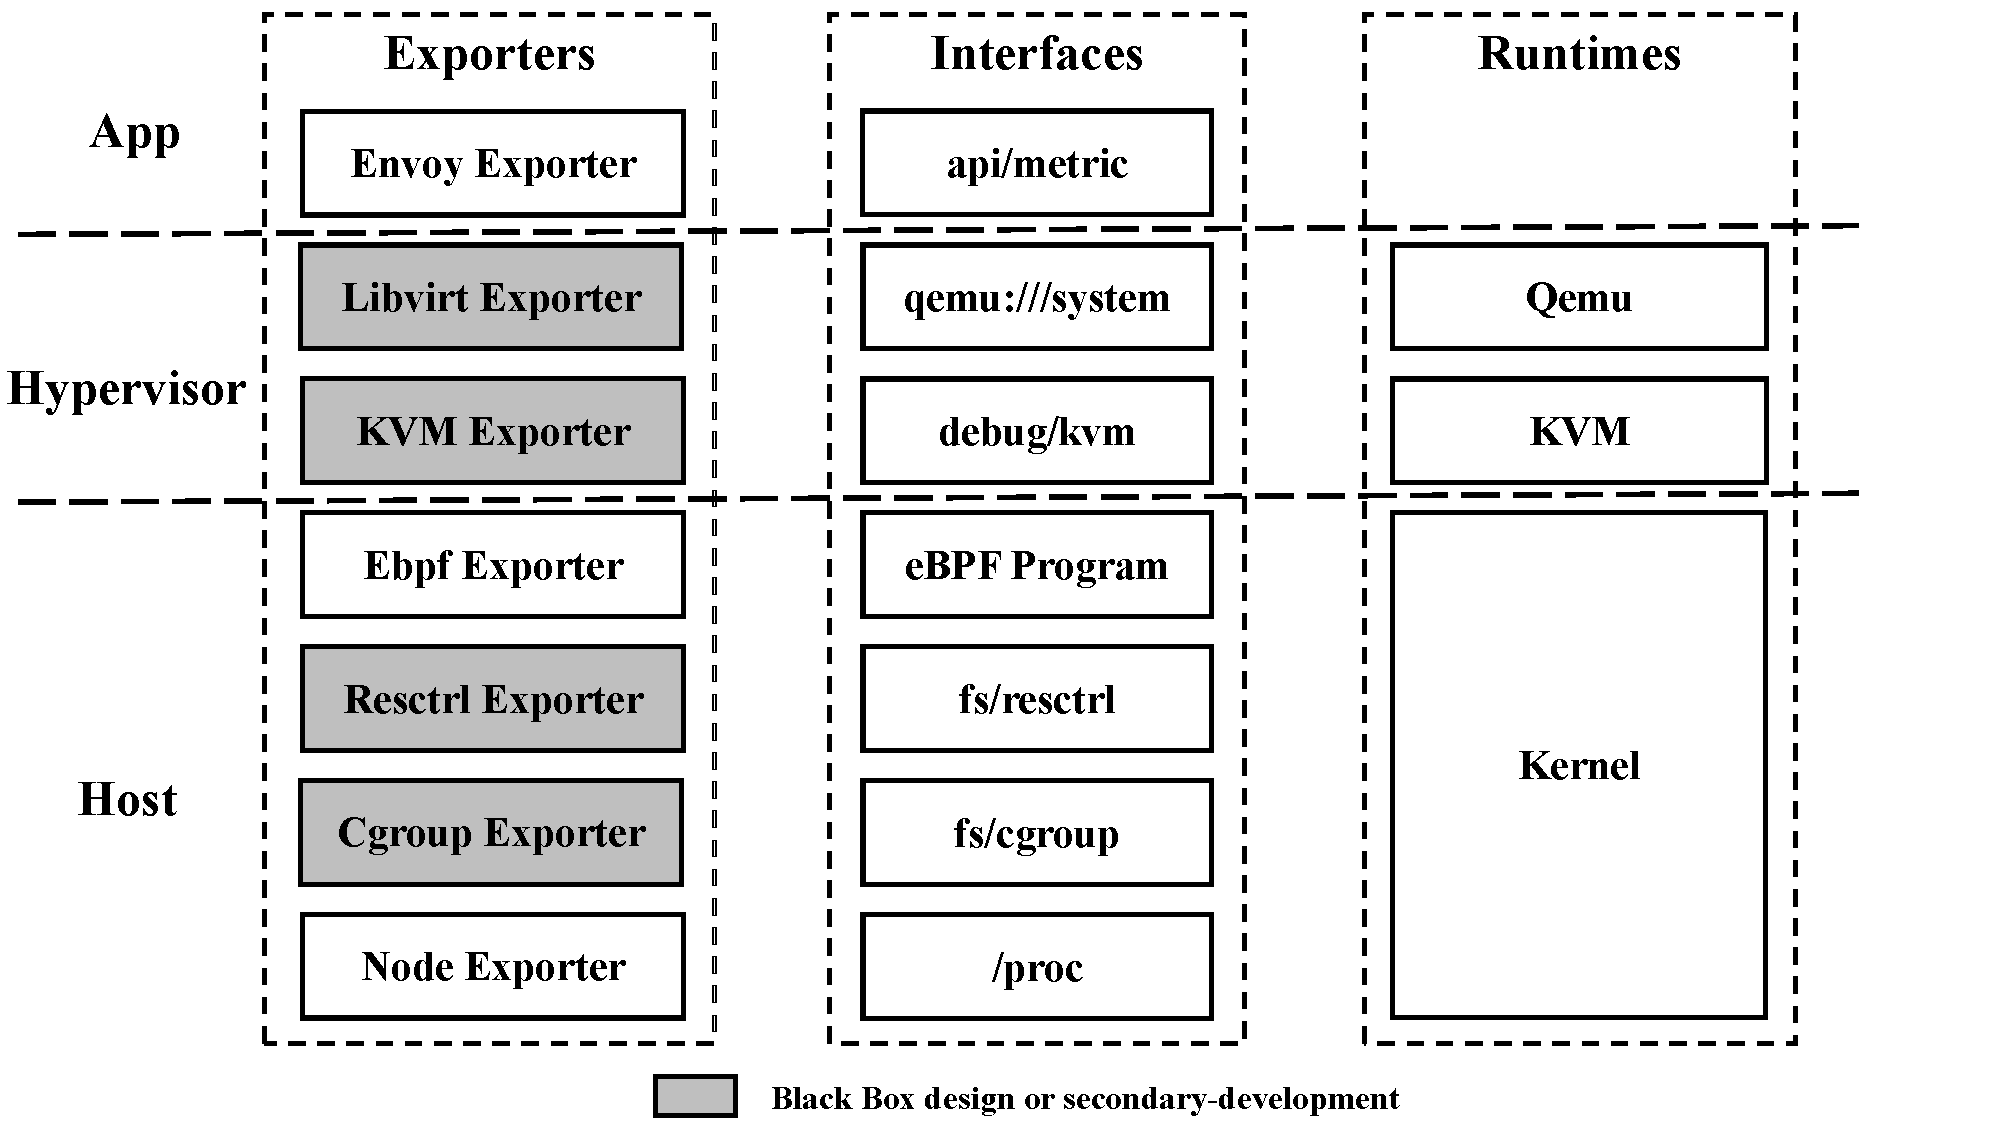
\includegraphics[width=0.8\textwidth]{exporters}
    \bicaption{\quad Exporters设计}{\quad Exporters Design}
    \label{fig:exporters} 
\end{figure}

可观测性系统中Observed的实现则包含了各个维度的Exporter的开发与配置。如图~\ref{fig:exporters}所示,Observed中包含了7种Exporter,能够在Host、Hypervisor、App三个维度围绕虚拟机提供丰富的数据采集,每个Exporter具体实现如下:

\begin{enumerate}
    \item \textbf{Envoy Exporter}:开源社区提供的一种L7代理和通信总线,面向大型现代服务架构设计,作为基础组件运行在各个Overlay Network系统中。Envoy的首要目的是构造透明网络,同时,为协助解决网络与应用层面的问题排查,Envoy还为各个代理子系统提供了强大的统计功能,统计功能支持大部分L7层传输协议,同时对于一些云原生应用,如Redis、Mysql等,能够进一步统计应用层协议的指标信息,如延迟、请求数等。
    
    \item \textbf{Libvirt Exporter}:Prometheus开源社区开发的监控组件,提供了Hypervisor维度的指标采集。Libvirt是一个统一的虚拟化接口层,提供了丰富的虚拟机管理选项,Libvirt Exporter基于Libvirt Monitor接口实现,能够采集虚拟机的各个设备的性能指标,如vCPU时间片、内存使用量、网络设备的吞吐量及IO设备的吞吐量等。Observed实现中为Libvirt Exporter增加的Perf Event监测功能,从而能够提供虚拟机粒度的性能事件指标信息,如cycles、instruction及cache miss等。
    
    \item \textbf{KVM Exporter}:本文实现了Hypervisor维度的指标采集。KVM内核模块提供了一个Debug文件系统,在最顶层的目录中,记录了内核模块的运行信息,如虚拟机陷出的总计数等,同时,对于每个虚拟机进程,还会创建对应的子目录,并以单个虚拟机为粒度记录内核模块的运行数据,最后,在每个虚拟机目录中,还会为每个vCPU创建一个目录,记录vCPU的时钟源相关信息。KVM Exporter基于上述机制实现,通过扫描Debug系统中的目录,并为遍历每个虚拟机条目来生成相关的指标信息,默认情况下使用虚拟机进程号作为标签,也允许传入一个配置文件,来实现虚拟机进程号与虚拟机名称之间的转化。

    \item \textbf{eBPF Exporter}:Cloudflare公司开发eBPF监控组件,提供了内核侧的自定义指标采集。eBPF Exporter能够加载用户编译为字节码的eBPF程序,并通过RingBuffer收集内核侧eBPF程序采集的数据转化为指标。Observed中实现了系统调用及vHost Net内核模块两个eBPF采集程序。内核中系统调用分布在各个子模块中,并通过注册系统调用的方式加入到系统调用表中,用户态应用发起的系统调用会触发一次中断,并最终进入系统调用分发函数。因此利用raw tracepoint机制在系统调用分发函数的开始与结束处进行eBPF插桩,就能够捕获系统调用的执行信息。如图~\ref{fig:syscall_hook}所示,当进程进入系统调用中时,通过BPF Helper函数获取当前task结构体指针,并读取进程号、Cgroup描述符等信息。随后,在x86架构下,通过Helper函数读取系统调用上下文中的ax寄存器,进一步获取当前的系统调用号。组合上述两种信息可以得到系统调用的基础信息。而在系统调用起始与结束处通过BPF Stack传递时间戳信息,在记录系统调用执行频率的同时,也能够进一步对执行时间进行统计。vHost Net内核模块的监测则围绕worker内核线程展开,如图~\ref{fig:vhost_net}所示,worker线程中可能执行4种不同的回调函数,分别用于虚拟机的网络发送与接受,通fentry机制在这些函数的入口与出口处进行插桩,就能够统计出各个函数执行频率以及延时等信息。

    \begin{figure}[H]
        \centering
        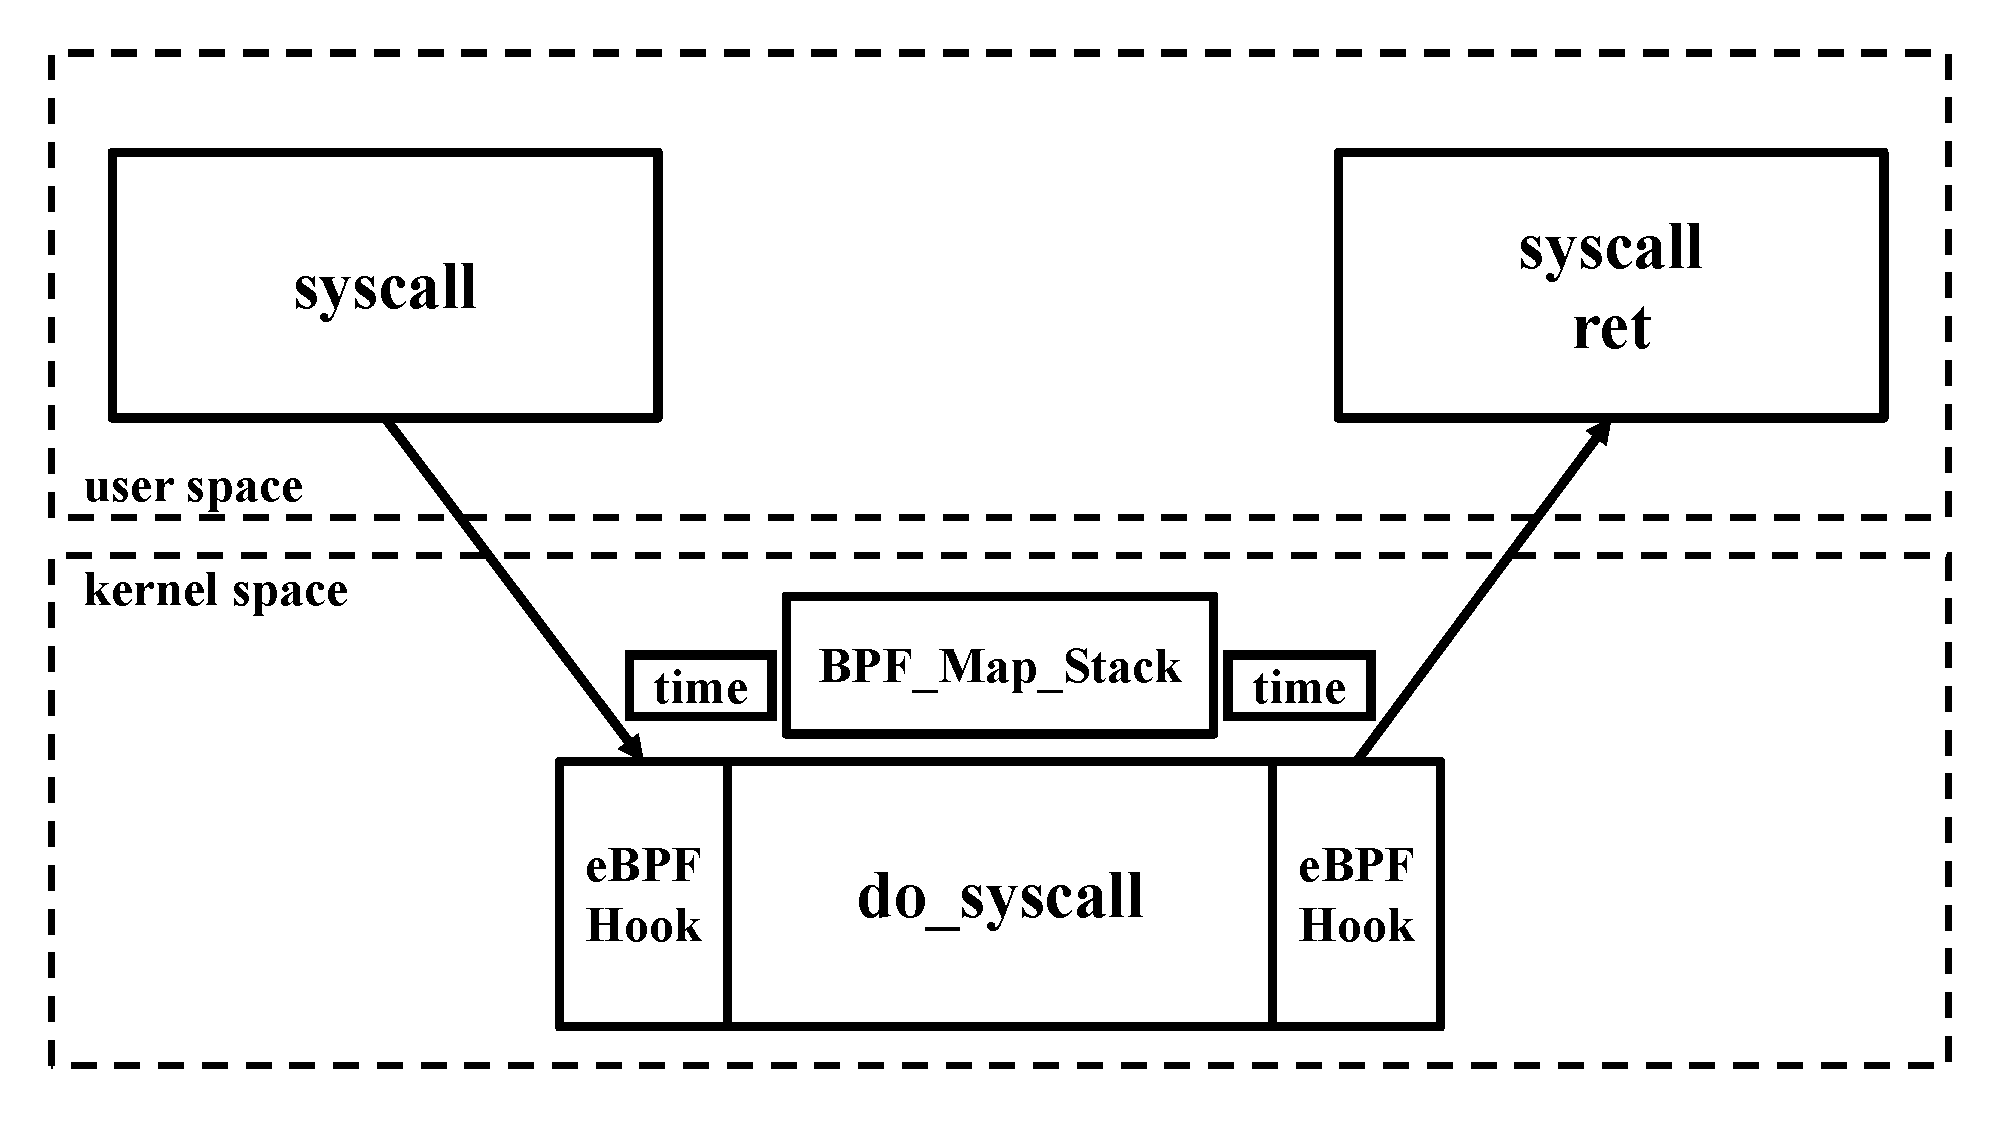
\includegraphics[width=0.6\textwidth]{syscall_hook}
        \bicaption{\quad eBPF Syscall插桩}{\quad eBPF Syscall Hooking}
        \label{fig:syscall_hook}
    \end{figure}

    \item \textbf{Resctrl Exporter}:本文实现了Resctrl子系统的指标采集。Intel RDT等硬件技术提供了进程粒度的CPU末级缓存与内存带宽的监测能力,Linux Resctrl作为这类技术的软件接口,提供了一个内核文件系统,用户可以通过在此文件系统中创建文件夹的形式来创建Monitor Group,而将进程加入到其中之后,Resctrl子系统就会开始为进程记录LLC与内存带宽信息。Resctrl Exporter基于Resctrl子系统实现, 通过扫描子系统中的Monitor Group来生成相关的指标信息,并将Monitor Group作为标签以便于后续聚合。
    
    \item \textbf{Cgroup Exporter}:Google开发的容器监控组件,提供Cgroup子系统的基础指标采集。Cgroup Exporter通过扫描cgroup文件系统,读取目标cgroup中各个控制子系统的记账信息,并生成指标信息,从而实现对于进程cgroup的监控。
    
    \item \textbf{Node Exporter}:Prometheus社区的基础监控组件,提供Host维度的基础指标采集。Node Exporter利用Linux内核提供的交互接口,包含系统调用、内存文件系统等,来获取Host各个子系统中的运行状态信息,如通过/proc内核文件系统,获取运行时间、内存信息等。Observed实现中使能了NodeExporter的Perf Event监测模块,模块支持采集Host上的性能事件,包括cycles、instruction及cache miss等。

\end{enumerate}

% 解释指标的具体含义(列举少数)
% 总体概述,然后:
% - Host
% - Hypervisor
% - App

实时可观测性系统采集的指标涵盖Host、Hypervisor、App三个层级,涉及CPU、Cache、Memroy、IO、Network等资源,原始指标数量达到344种。

\begin{enumerate}
    \item \textbf{Host层级指标}:如表~\ref{tab:host_metric}所示, 指标来源分别为Kernel、
eBPF与Resctrl子系统。从Kernel采集的指标通常为总体性的资源指标,在CPU资源上,首先从时间记账子系统中采集了Host总体CPU时间片的分布,如sys\_time、user\_time,同时也从设备的角度采集了每个CPU的基准频率、最高频率与实时频率等信息。在内存资源上,主要从内存子系统中采集了Host上内存资源的使用情况,如内存使用量、可用内存量、swap可用量等。在网络资源上,首先针对每个物理设备采集驱动记录的transmit、receive等收发包信息,同时,针对目标进程采集了tcp、udp等描述符的使用情况。在磁盘IO资源上,针对每个存储设备采集驱动记录的read、write统计信息等。从eBPF采集的指标是作为Kernel指标的扩展,首先针对系统调用,以Cgroup为粒度统计系统调用的使用频次、执行时间等信息,其次针对驱动程序,如vHost Net虚拟网络设备后端,以Cgroup为粒度统计Worker执行回调函数的频次与时间。从Resctrl采集的指标在Host维度主要包含各个Numa实时的LLC使用率以及内存带宽大小。

\begin{table}[!htbp]
    \bicaption{\quad Host层级指标}{\quad Host Metric list}% caption
    \label{tab:host_metric}
    \footnotesize% fontsize
    \setlength{\tabcolsep}{4pt}% column separation
    \renewcommand{\arraystretch}{1.25}% ro w space 
    \centering
    \begin{tabular}{ll}
        \hline
        %\multicolumn{num_of_cols_to_merge}{alignment}{contents} \\
        %\cline{i-j}% partial hline from column i to column j
        来源 & 指标\\
        \hline
        Kernel(271) & [cpu] sys\_time、user\_time、freq ... \\
        & [mem] usage、avail、swapfree、bounce、hugepage ...\\
        & [network] transmit、netstat、sockstat、ip、speed ...\\
        & [disk]flush requests、flush request time、read、write ...\\
        & ...\\
        eBPF(2) & [syscall] count、duration\\
        Resctrl(3) & llc cap、mem b/w local、mem b/w total\\
        \hline
    \end{tabular}
\end{table}

    \item \textbf{Hypervisor层级的指标}:如表~\ref{tab:hypervisor_metric}所示,指标来源分别为Libvirt与KVM。从Libvirt采集的指标通常为虚拟机粒度的资源指标,在CPU资源上,一方面从进程角度采集vCPU的时间记账以及调度子系统中的等待时间和调度延迟,另一方面从虚拟机角度采集vCPU内核态与用户态的时间片分布。在Cache资源上,利用Resctrl子系统提供的观测能力,采集虚拟机进程及子进程在LLC与内存带宽上的使用情况。在内存资源上,从ballon内存驱动上采集虚拟机内存资源的使用情况,包括内存总量、可用内存量、磁盘Cache总量以及虚拟机内存fault计数等。在网络资源上,采集虚拟网卡的transmit与receive信息。在磁盘IO资源上,采集虚拟磁盘设备的read、write数量以及read request、write request、flush request计数等。同时考虑虚拟机的进程特性采集Perf指标,性能事件包括Instruction、Branch Instruction、CPI, Cache Miss、Context Switch等。从KVM采集的指标通常描述虚拟机的状态,如针对虚拟机进程描述符,采集虚拟机的陷出事件,包含vm\_exit、io\_exit、irq\_exit等,而针对vCPU描述符,则采集时间子系统上的偏移等信息。

\begin{table}[!htbp]
    \bicaption{\quad Hypervisor层级指标}{\quad Hypervisor Metric list}% caption
    \label{tab:hypervisor_metric}
    \footnotesize% fontsize
    \setlength{\tabcolsep}{4pt}% column separation
    \renewcommand{\arraystretch}{1.25}% row space 
    \centering
    \begin{tabular}{ll}
        \hline
        %\multicolumn{num_of_cols_to_merge}{alignment}{contents} \\
        %\cline{i-j}% partial hline from column i to column j
        来源 & 指标\\
        \hline
        Libvirt(68) & [vcpu] sys\_time、user\_time、wait、delay...\\
        & [mem] usable、avail、dick cache、rss ...\\
        & [perf] cycle、instruction、cache miss ...\\
        & [block] flush request、flush time、read、write ...\\
        & [interface] receive、transmit ...\\
        & ...\\
        KVM(59) & vm\_exit、io\_exit、irq\_exit、irq\_inject、halt\_poll ...\\
        \hline
    \end{tabular}
\end{table}

    \item \textbf{App层级的指标}:主要从日志、内嵌的指标采集接口以及Envoy网络代理上采集。以Redis为例,通过Envoy网络代理接管传入Redis的所有流量,并在代理中记录各种操作的数量、延时统计等信息。
    
\end{enumerate}

\section{基准性能实验设计与分析}

\subsection{基准性能实验设计}

实验中使用两台C6服务器作为Client和Server,服务器具体配置如表~\ref{tab:c6_info}所示,其中Client服务器额外承担实验管理的功能,同时作为Observer角色部署Prometheus Server等组件,而Server主要承载具体的应用,同时作为Observed角色部署上述设计实现的6种Exporter,并为Exporter设置Numa亲和性以避免对应用产生干扰。基准性能实验测试无干扰情况下各个典型应用的基础性能,并使用华为云提供的竖亥Benchmark来模拟真实场景下的应用负载。

\begin{table}[!htbp]
    \bicaption{\quad C6服务器信息}{\quad C6 Information}% caption
    \label{tab:c6_info}
    \footnotesize% fontsize
    \setlength{\tabcolsep}{4pt}% column separation
    \renewcommand{\arraystretch}{1.25}% row space 
    \centering
    \begin{tabular}{lc}
        \hline
        类型 & 信息 \\
        \hline
        OS & Ubuntu 22.04 ( Kernel 5.15.0) \\
        CPU & Intel Xeon Gold 6151 (18 cores) * 2 \\
        Processor Core Frequency & 3GHz,Turbo 3.4GHz \\
        L1 Caches & 32KB *,  8-way set associative, split D/I \\
        L2 Caches & 1024KB, 16-way set associative \\
        L3 Caches & 25344KB, 11-way set associative \\
        Main Memory & 32GB * 12, 2666MHz DDR4 \\
        Storage & Avago MegaRAID, 2.18T SAS RAID0, 87.322T SATA RAID0 \\
        NIC & Intel Corporation Ethernet Connection X722 for 10GbE SFP+(10Gbit) \\
        \hline
    \end{tabular}
\end{table}

% 1)Redis、Memcached。使用memtier_benchmark来产生负载,负载的模型由华为云提供,包括Normal、Random两类模拟负载

% 2)Mysql。使用TPCC作为基准实验负载

% 3)Elasticsearch。使用YCSB作为基准负载

% 4)Kafka。

% 5)Nginx。

% 6)Render。使用华为内部的模拟负载。

\subsection{典型应用资源倾向分析}

无干扰实验中计算各个监测指标的变异系数,得到不同应用对应的资源指标如图~\ref{fig:resource_affinity}所示。

\begin{figure}[H]
    \centering
    \begin{subfigure}[b]{0.49\textwidth}
      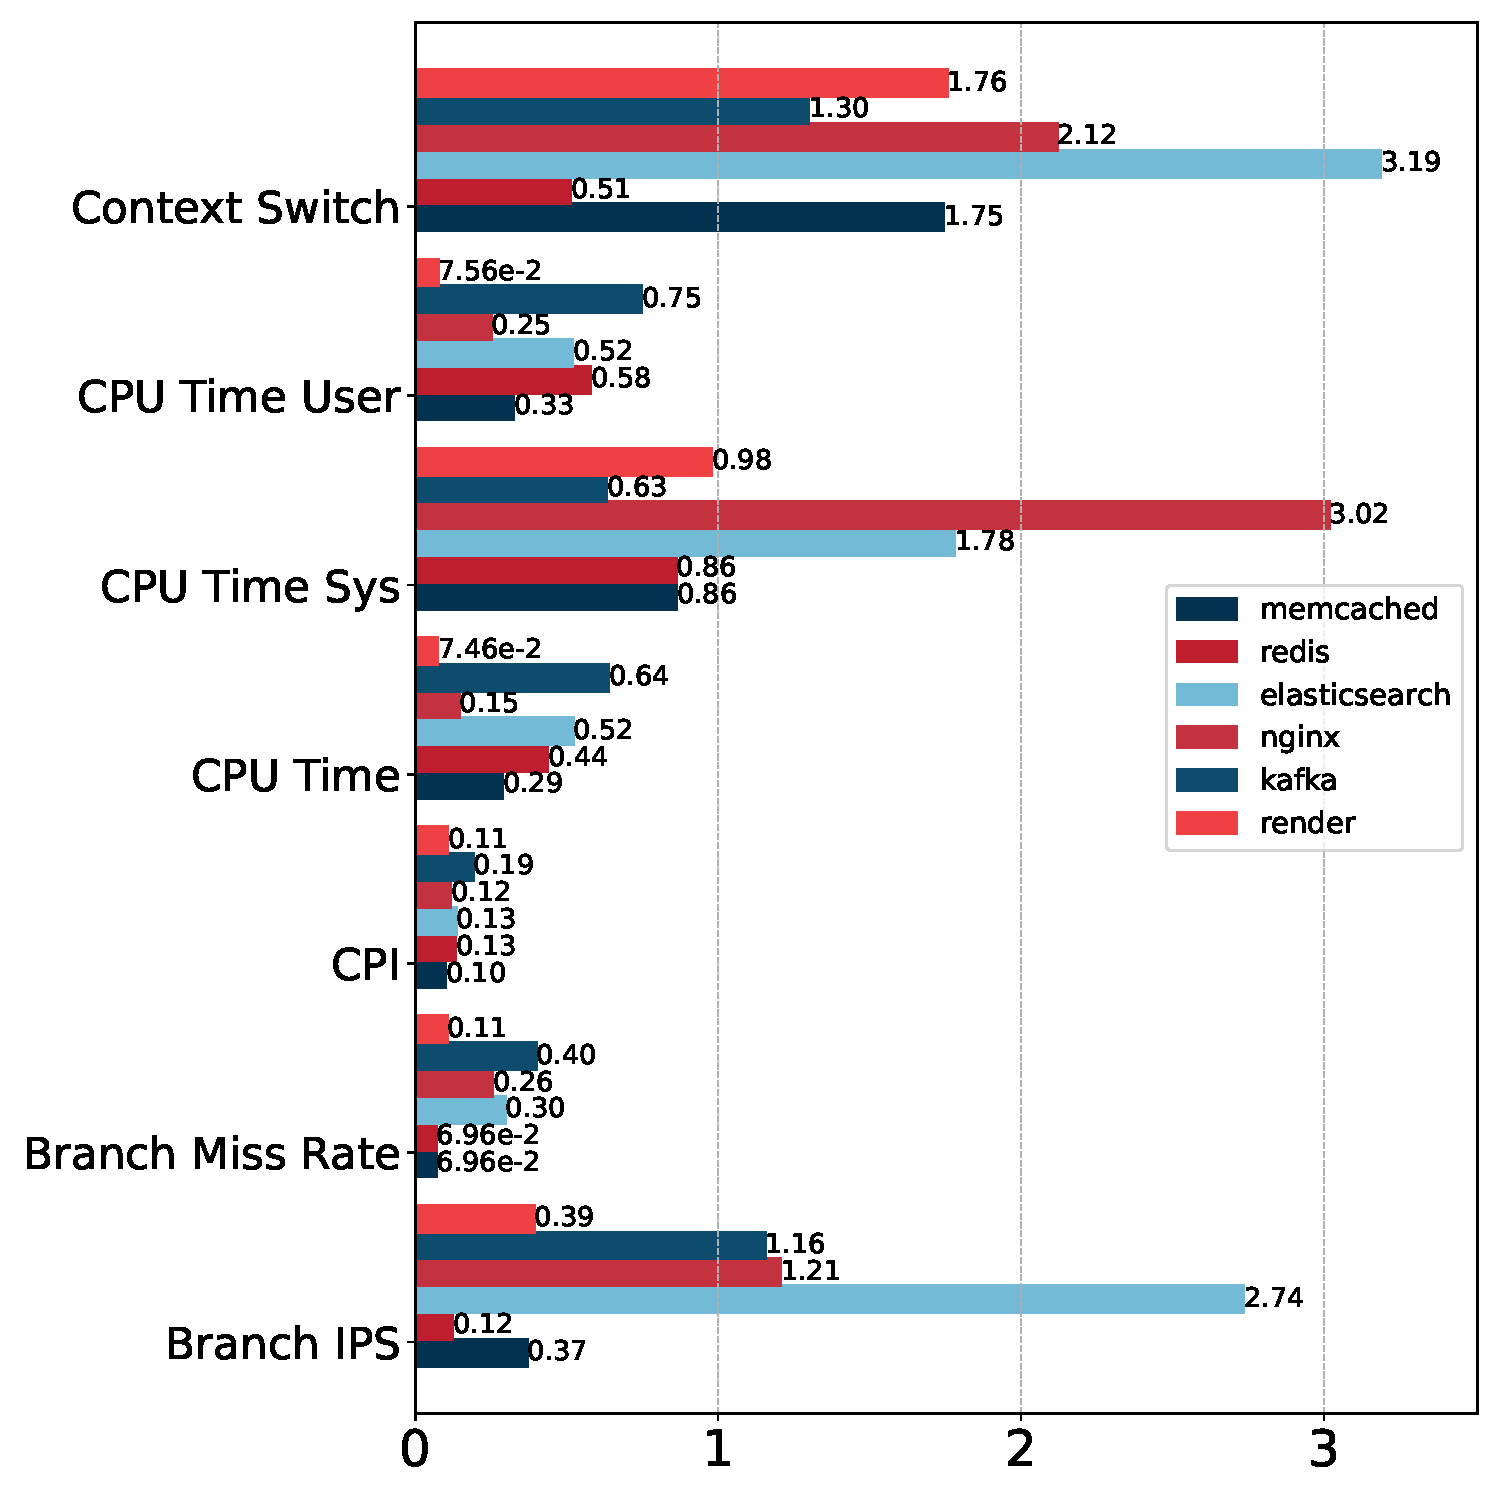
\includegraphics[width=\textwidth]{cof_cpu}
      \caption{CPU资源指标}
      \label{fig:cof_cpu}
    \end{subfigure}
    \begin{subfigure}[b]{0.49\textwidth}
        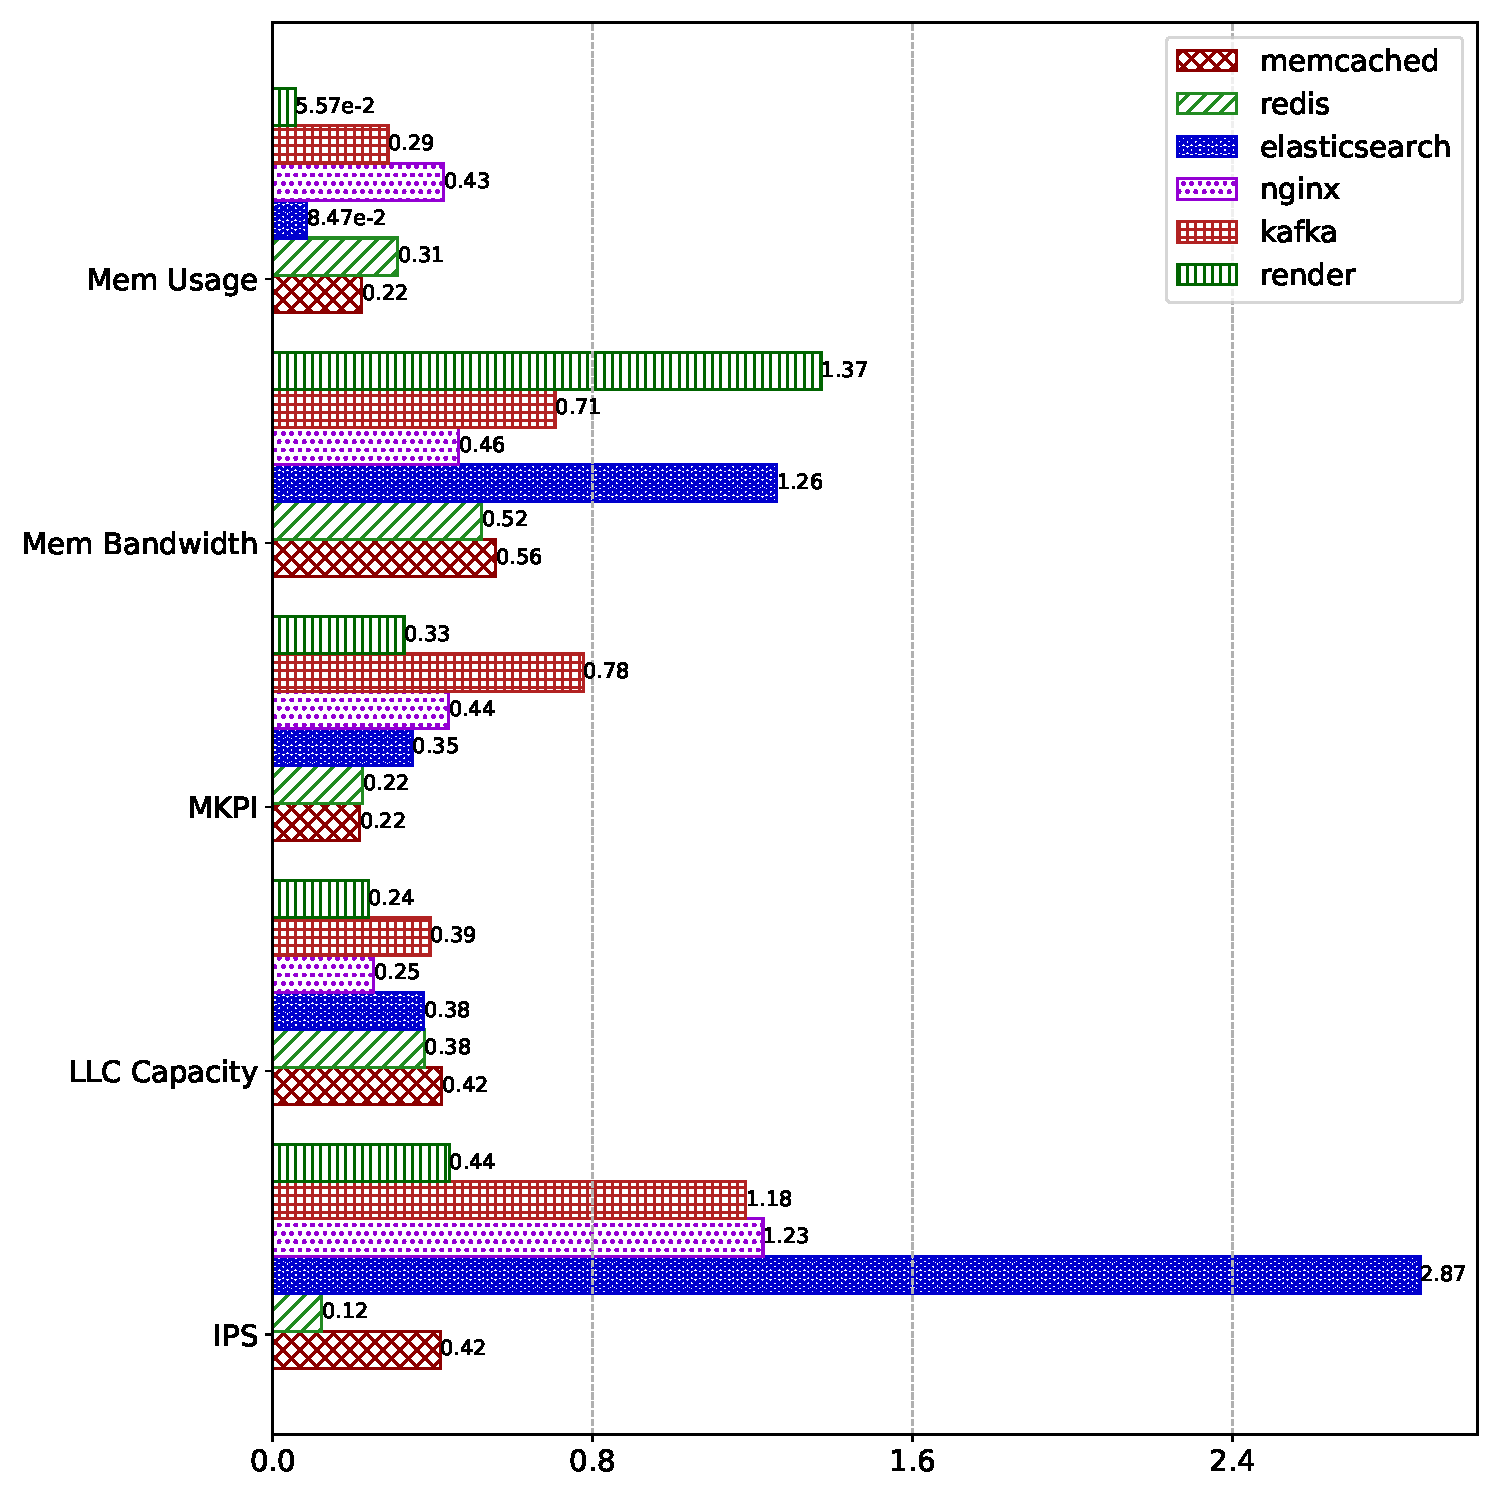
\includegraphics[width=\textwidth]{cof_mem}
        \caption{Cache、内存资源指标}
        \label{fig:cof_mem}
    \end{subfigure}
    \begin{subfigure}[b]{0.49\textwidth}
        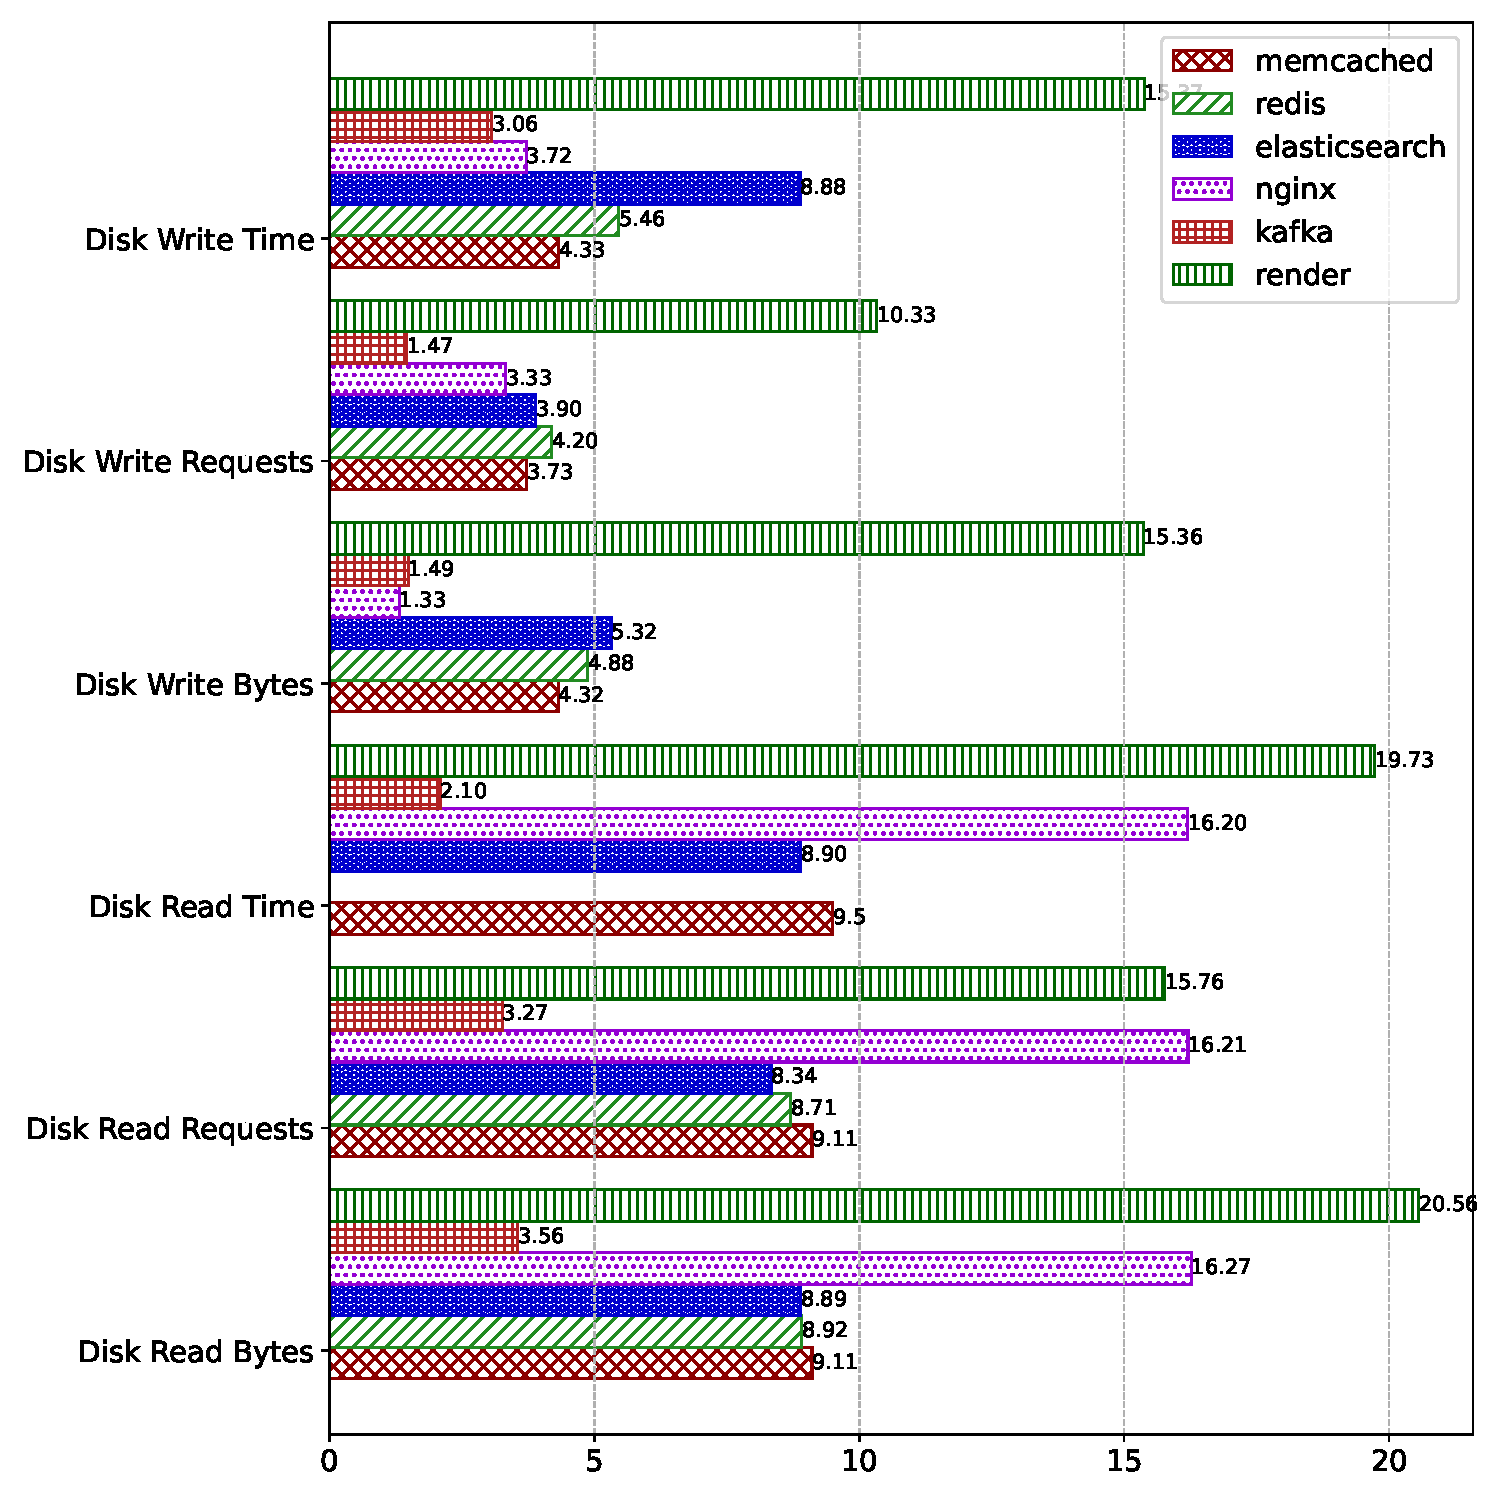
\includegraphics[width=\textwidth]{cof_io}
        \caption{IO资源指标}
        \label{fig:cof_mem}
    \end{subfigure}
    \begin{subfigure}[b]{0.49\textwidth}
        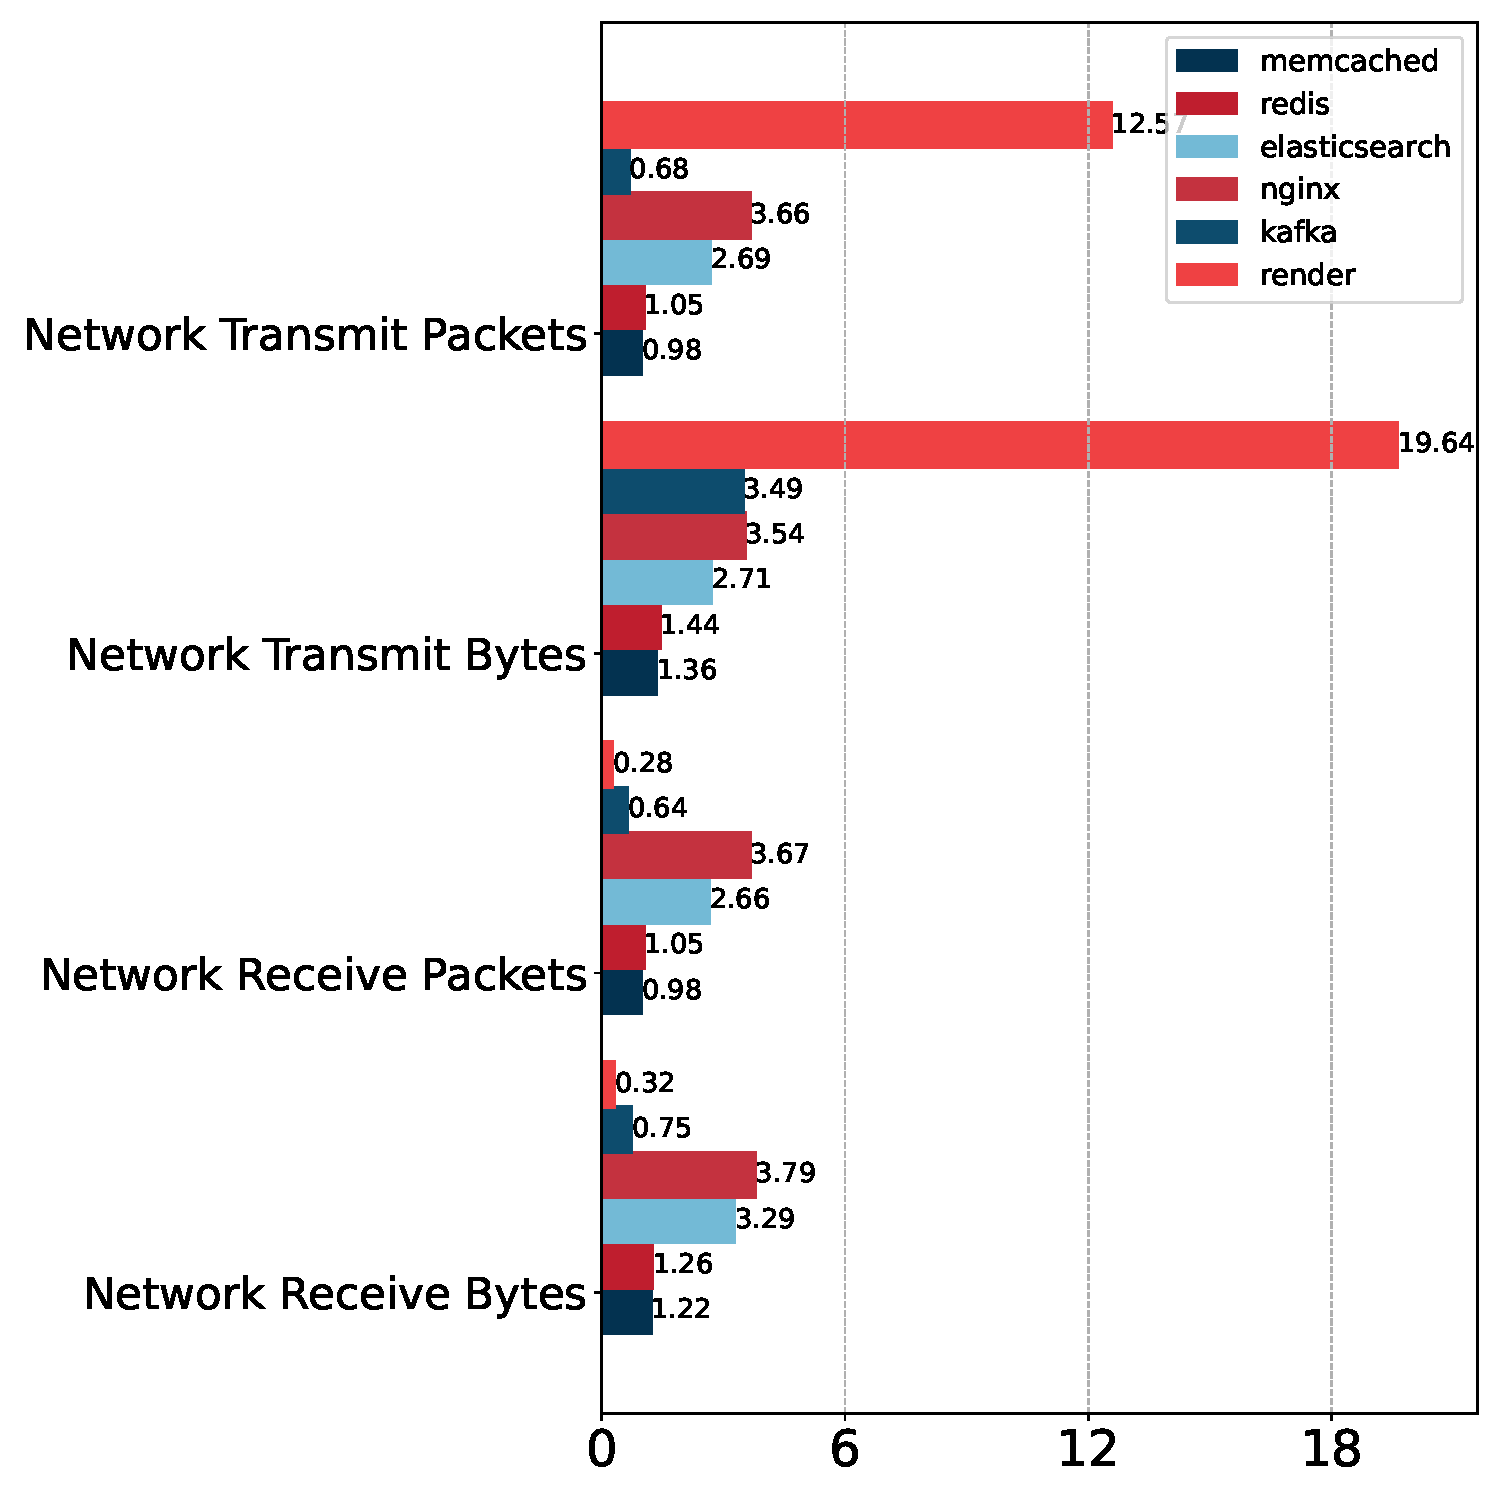
\includegraphics[width=\textwidth]{cof_network}
        \caption{网络资源指标}
        \label{fig:cof_mem}
    \end{subfigure}
\bicaption{\quad 总资源变异系数}{\quad Coefficient of Variation of Total Resources}
\label{fig:resource_affinity}
\end{figure}

从整体上看,Block I/O与Network I/O两类指标在不同应用之间呈现出较大的差异,相同指标在不同应用中的极大值与极小值差异可达$10^4$--$10^5$倍,而其余指标的差异通常不会超过20倍,这就导致图中一部分应用I/O相关指标非常高,而另一部分应用的相同指标则始终为一个较低的值。而在其他指标上则没有体现明显的差异度,这有如下两方面原因,首先,对于"利用率"类型的指标,这些指标存在明确的上下界,同时数值上的差异度难以直接体现,如对于CPU利用率,80\%与90\%利用率仅有约12\%的数值差异,但计算空闲CPU占比,则前者是后者的200\%,对于这些指标不能简单地使用差异度度量。其次,一些与硬件相关的指标波动不明显,如CPI,其波动通常受到流水线周期、指令阻塞和回退的数量等因素影响,在优化较好的现代处理器平台上,通常只会在一个较小的范围内波动。

具体到应用的差异性如图~\ref{fig:resource_affinity_0}所示,不同应用对于主要的5种系统资源的需求呈现处较大的差异:

\begin{figure}[H]
    \centering
    \begin{subfigure}[b]{0.85\textwidth}
      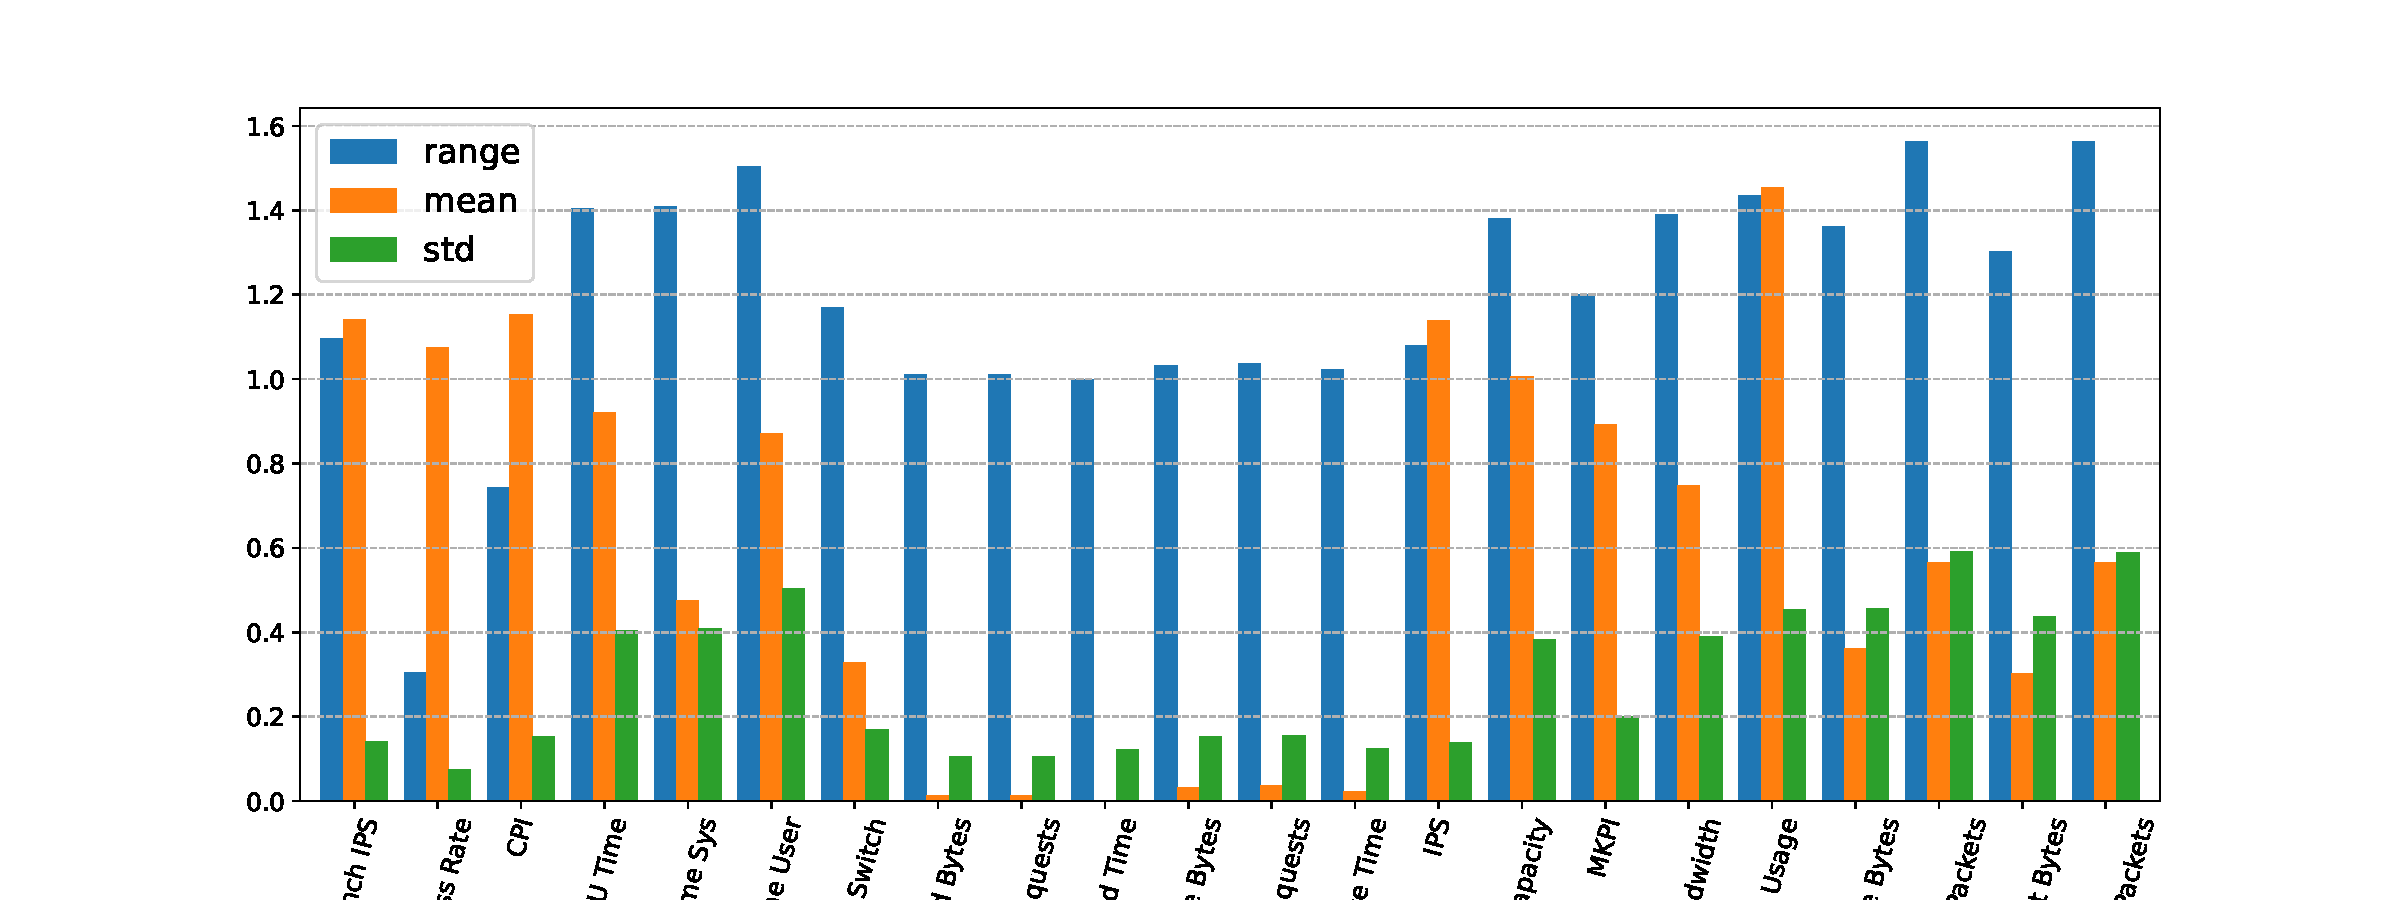
\includegraphics[width=\textwidth]{profile_redis}
      \caption{Redis资源使用}
      \label{fig:profile_redis}
    \end{subfigure}
    \begin{subfigure}[b]{0.85\textwidth}
        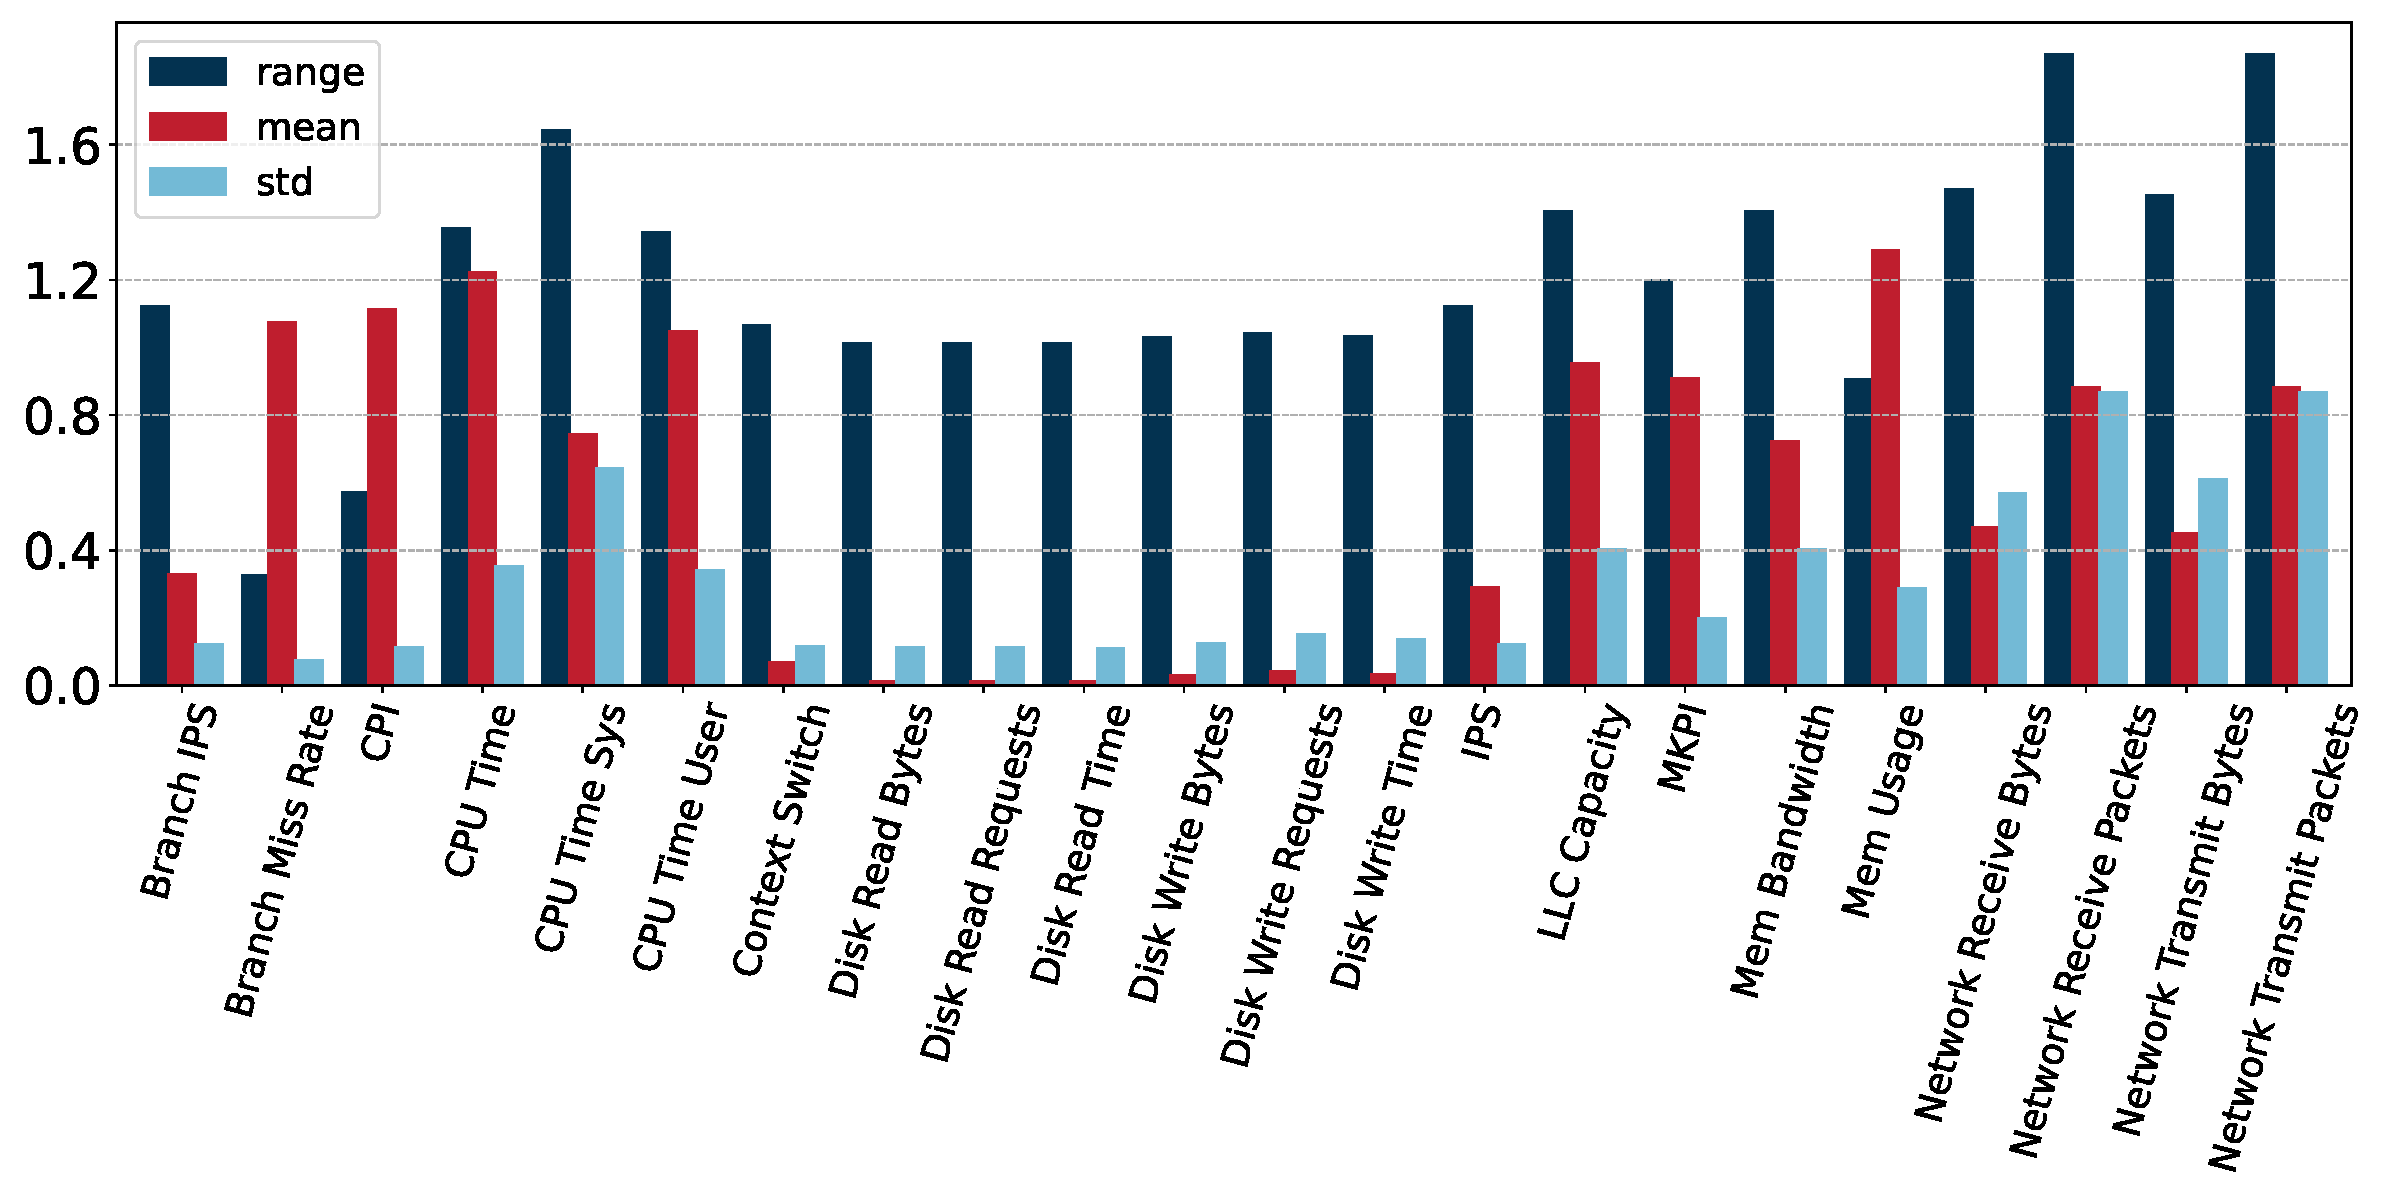
\includegraphics[width=\textwidth]{profile_memcached}
        \caption{Memcached资源使用}
        \label{fig:profile_memcached}
    \end{subfigure}
\bicaption{\quad Redis与Memcached资源使用情况}{\quad Resource Usage of Redis and Memcached}
\label{fig:resource_affinity_0}
\end{figure}

\begin{enumerate}
    \item \textbf{CPU资源}:应用的运行都需要CPU资源, 而不同应用对于CPU资源的使用上存在差异。Kafka运行时需要较多的CPU资源,体现在较高的IPS指标上。Redis、Memcached同样对于CPU资源有较高需求,从较多的平均CPU时间片占用能够看出,但不同之处在于,Redis、Memcached对于CPU资源的使用与请求强相关,在请求量较低时,由于频繁的睡眠与唤醒,此时不仅CPU资源需求少,同时CPI也较高,而当请求量足够多时,由于都基于epoll实现,因此密集的请求使得两者总是能够保持CPU的占用,而相较于Redis,Memcached在默认配置下更能够利用多核优势。Render应用同样需要较多的CPU资源,但与上述应用不同的是,Render在CPU资源使用上相当稳定,这一特点反映在较低的Branch IPS及Context Switch指标上。

\begin{figure}[H]
    \centering
    \begin{subfigure}[b]{0.85\textwidth}
      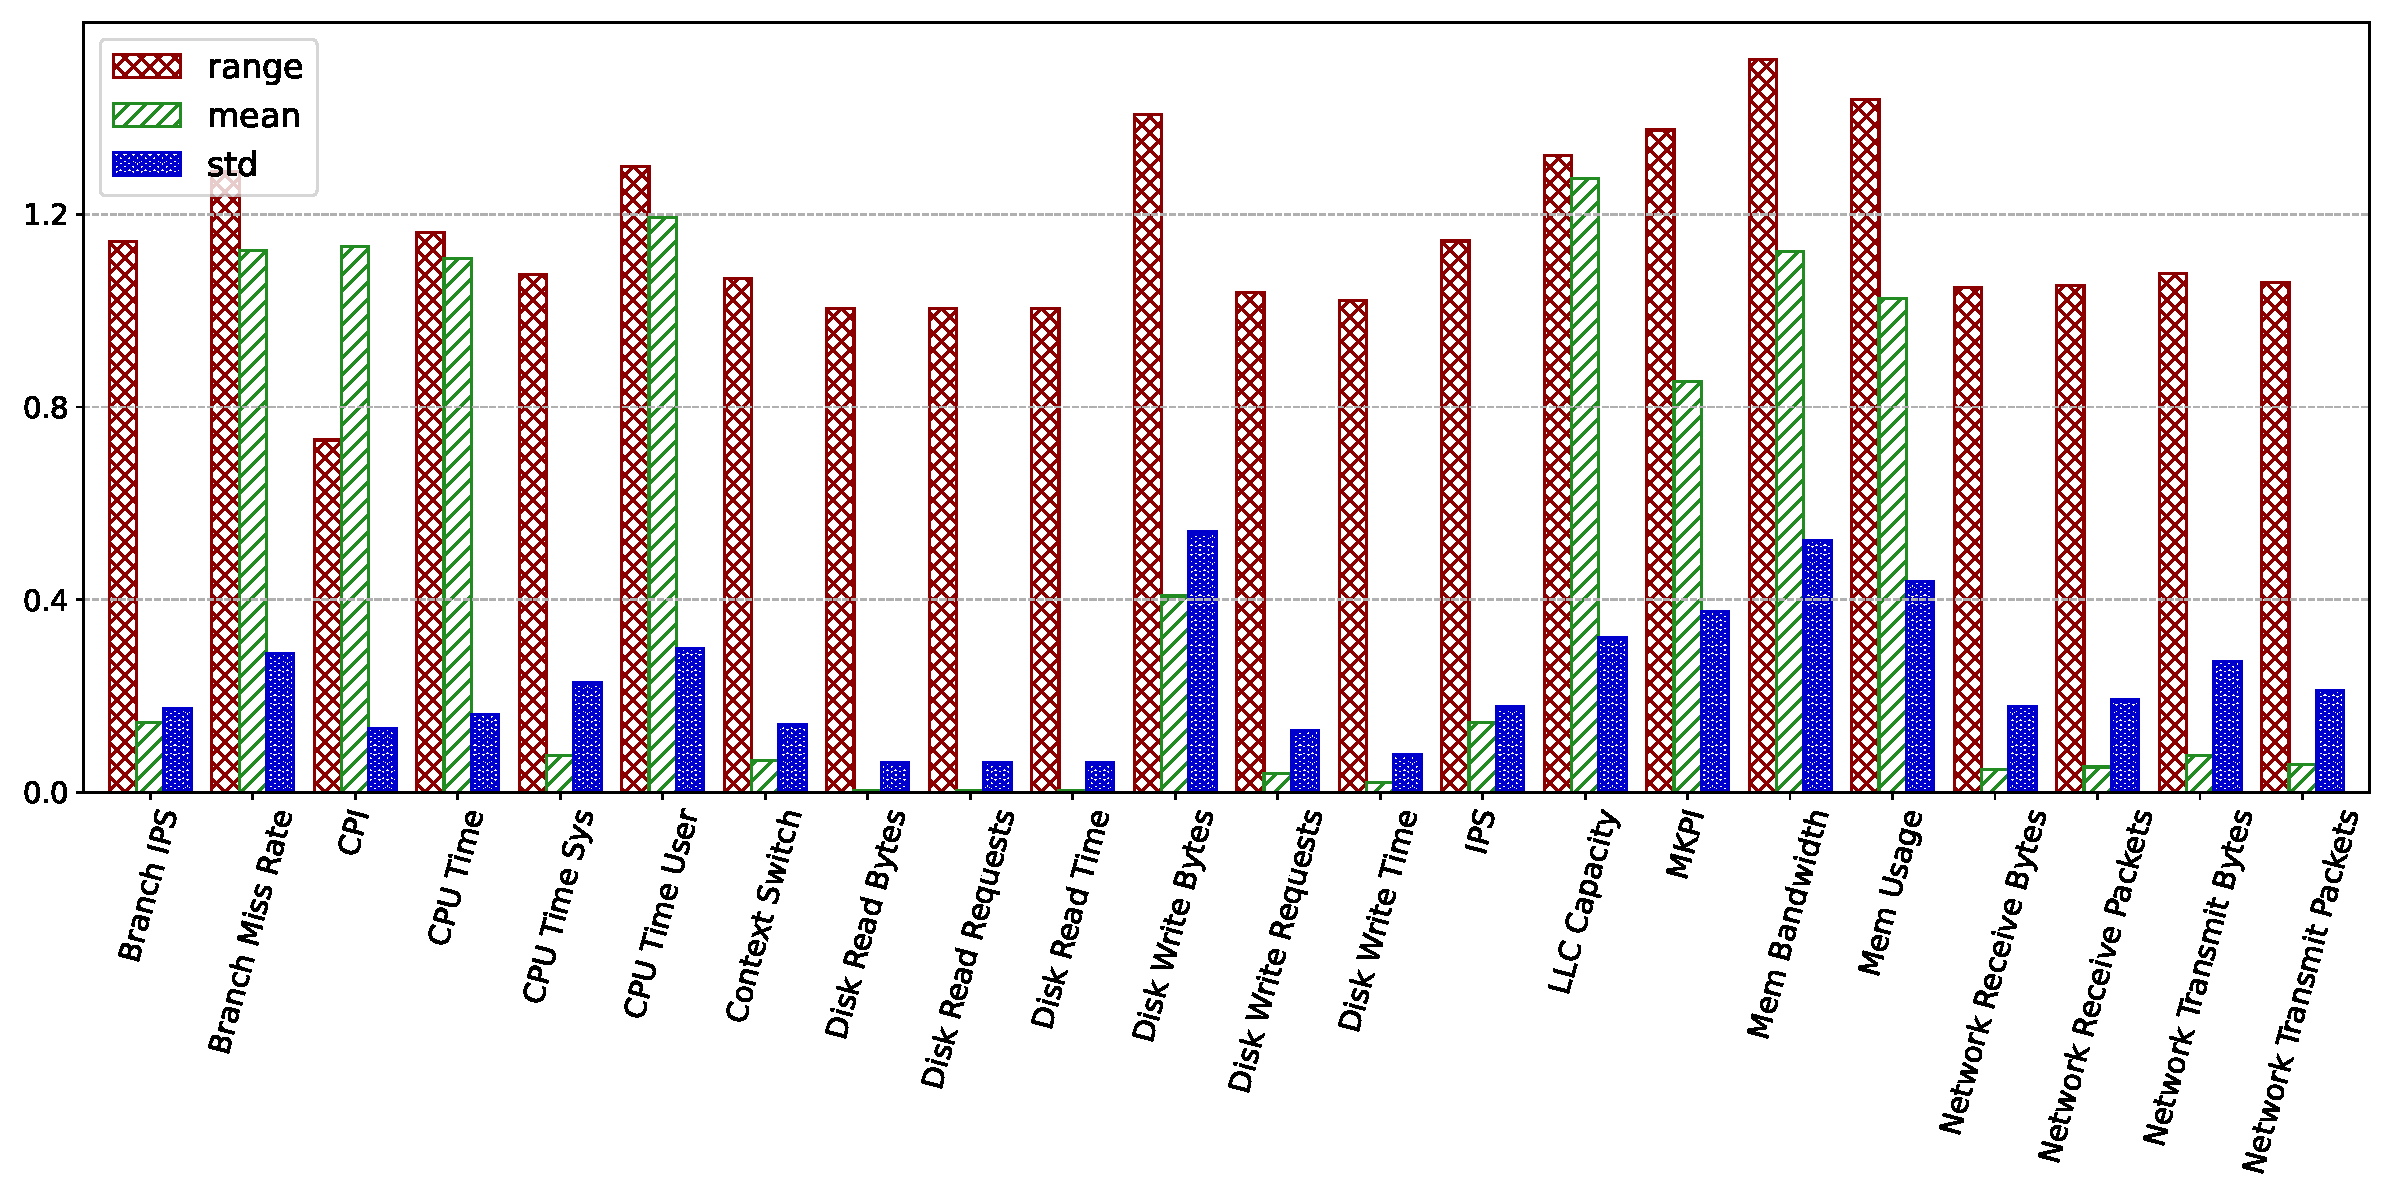
\includegraphics[width=\textwidth]{profile_nginx}
      \caption{Nginx资源使用}
      \label{fig:profile_nginx}
    \end{subfigure}
    \begin{subfigure}[b]{0.85\textwidth}
        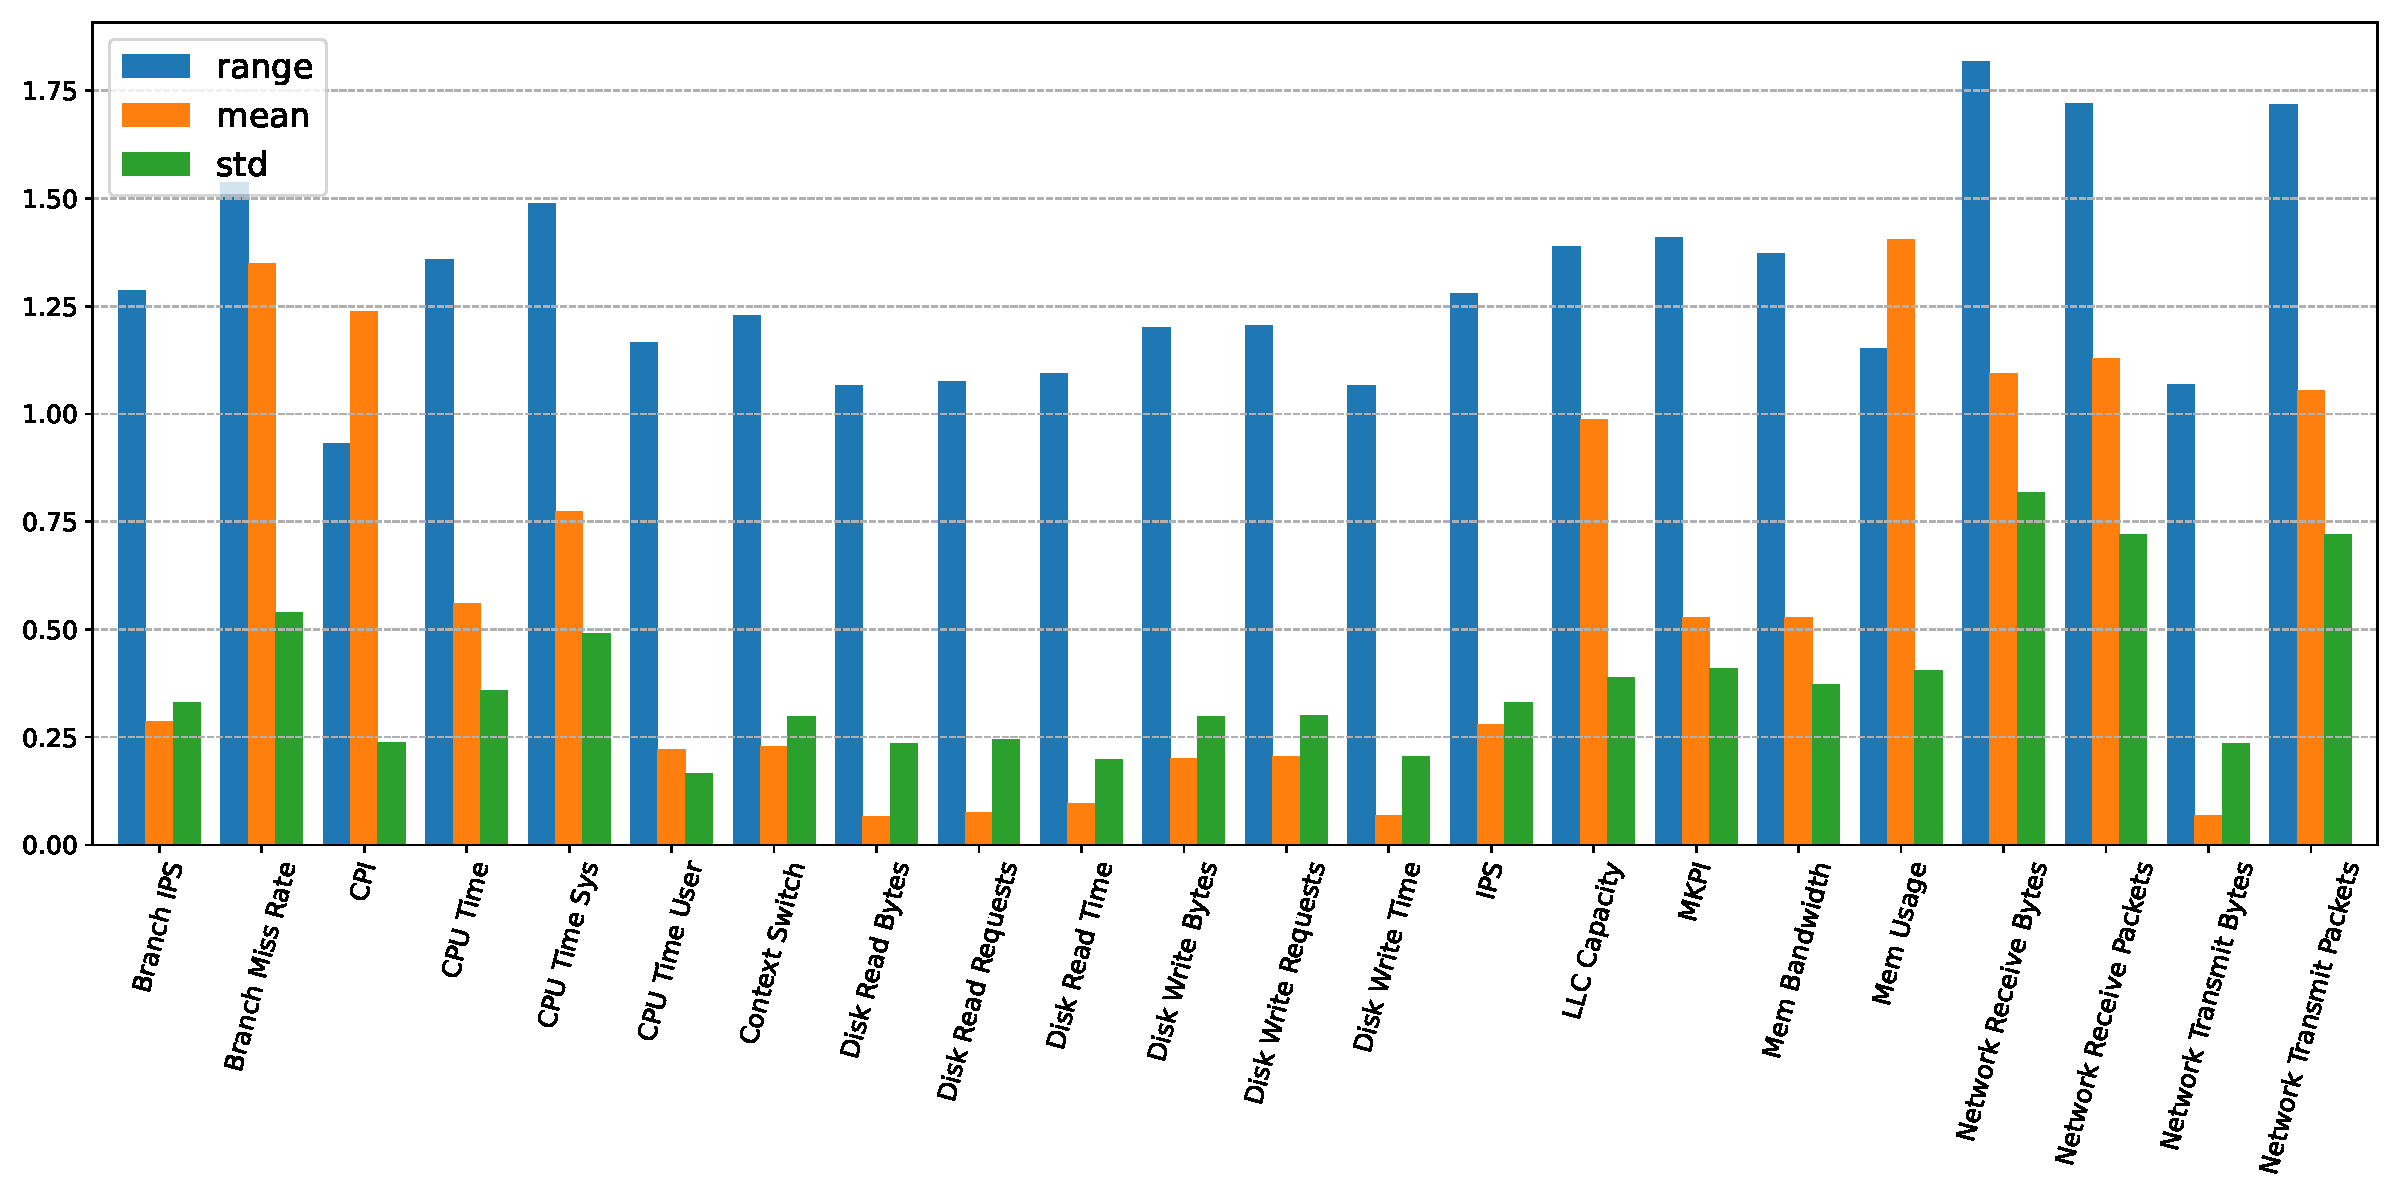
\includegraphics[width=\textwidth]{profile_kafka}
        \caption{Kafka资源使用}
        \label{fig:profile_kafka}
    \end{subfigure}
\bicaption{\quad Nginx与Kafka资源使用情况}{\quad Resource Usage of Nginx and Kafka}
\label{fig:resource_affinity_1}
\end{figure}


    \item \textbf{Cache资源}:末级缓存资源与内存访问强相关,分析不同应用的LLC相关指标,可以将应用按访存局部性进行划分,其中Nginx属于局部性较好的应用,其在运行过程中LLC使用率波动不明显,并且LLC Miss数量较少。而对于Redis、Memcached这类键值存储型应用,局部性则与工作负载相关,在随机负载下局部性表现较差,而在模拟负载下局部性则相对较好。
    
    \item \textbf{Memory资源}:内存资源区分带宽与使用量。典型应用中,Nginx在模拟负载下对内存带宽的需求较高,这点与其在Cache资源需求上的表现一致,其余应用则采用间歇与分批的内存读取,因此不会占用过多的内存带宽。内存使用量上,典型应用的内存占用除自身所需外,都与工作负载相关,华为云的默认负载下各个应用都会占用一定量的内存,没有特别的规律性。
    
    \item \textbf{Network资源}:在网络资源上,不同的应用使用需求差异很大,其中Redis、Memcached、Kafka表现出极高的网络需求,事实上这些应用都是服务型应用或自身就是网络消息中间件。而Elasticsearch、Render等在网络资源的需求上则相对较少,其中Elasticsearch并非不使用网络,因为工作负载中并没有长时间且持续性的请求,Render则是离线应用,因此几乎不会使用到网络资源。

\begin{figure}[H]
    \centering
    \begin{subfigure}[b]{0.85\textwidth}
      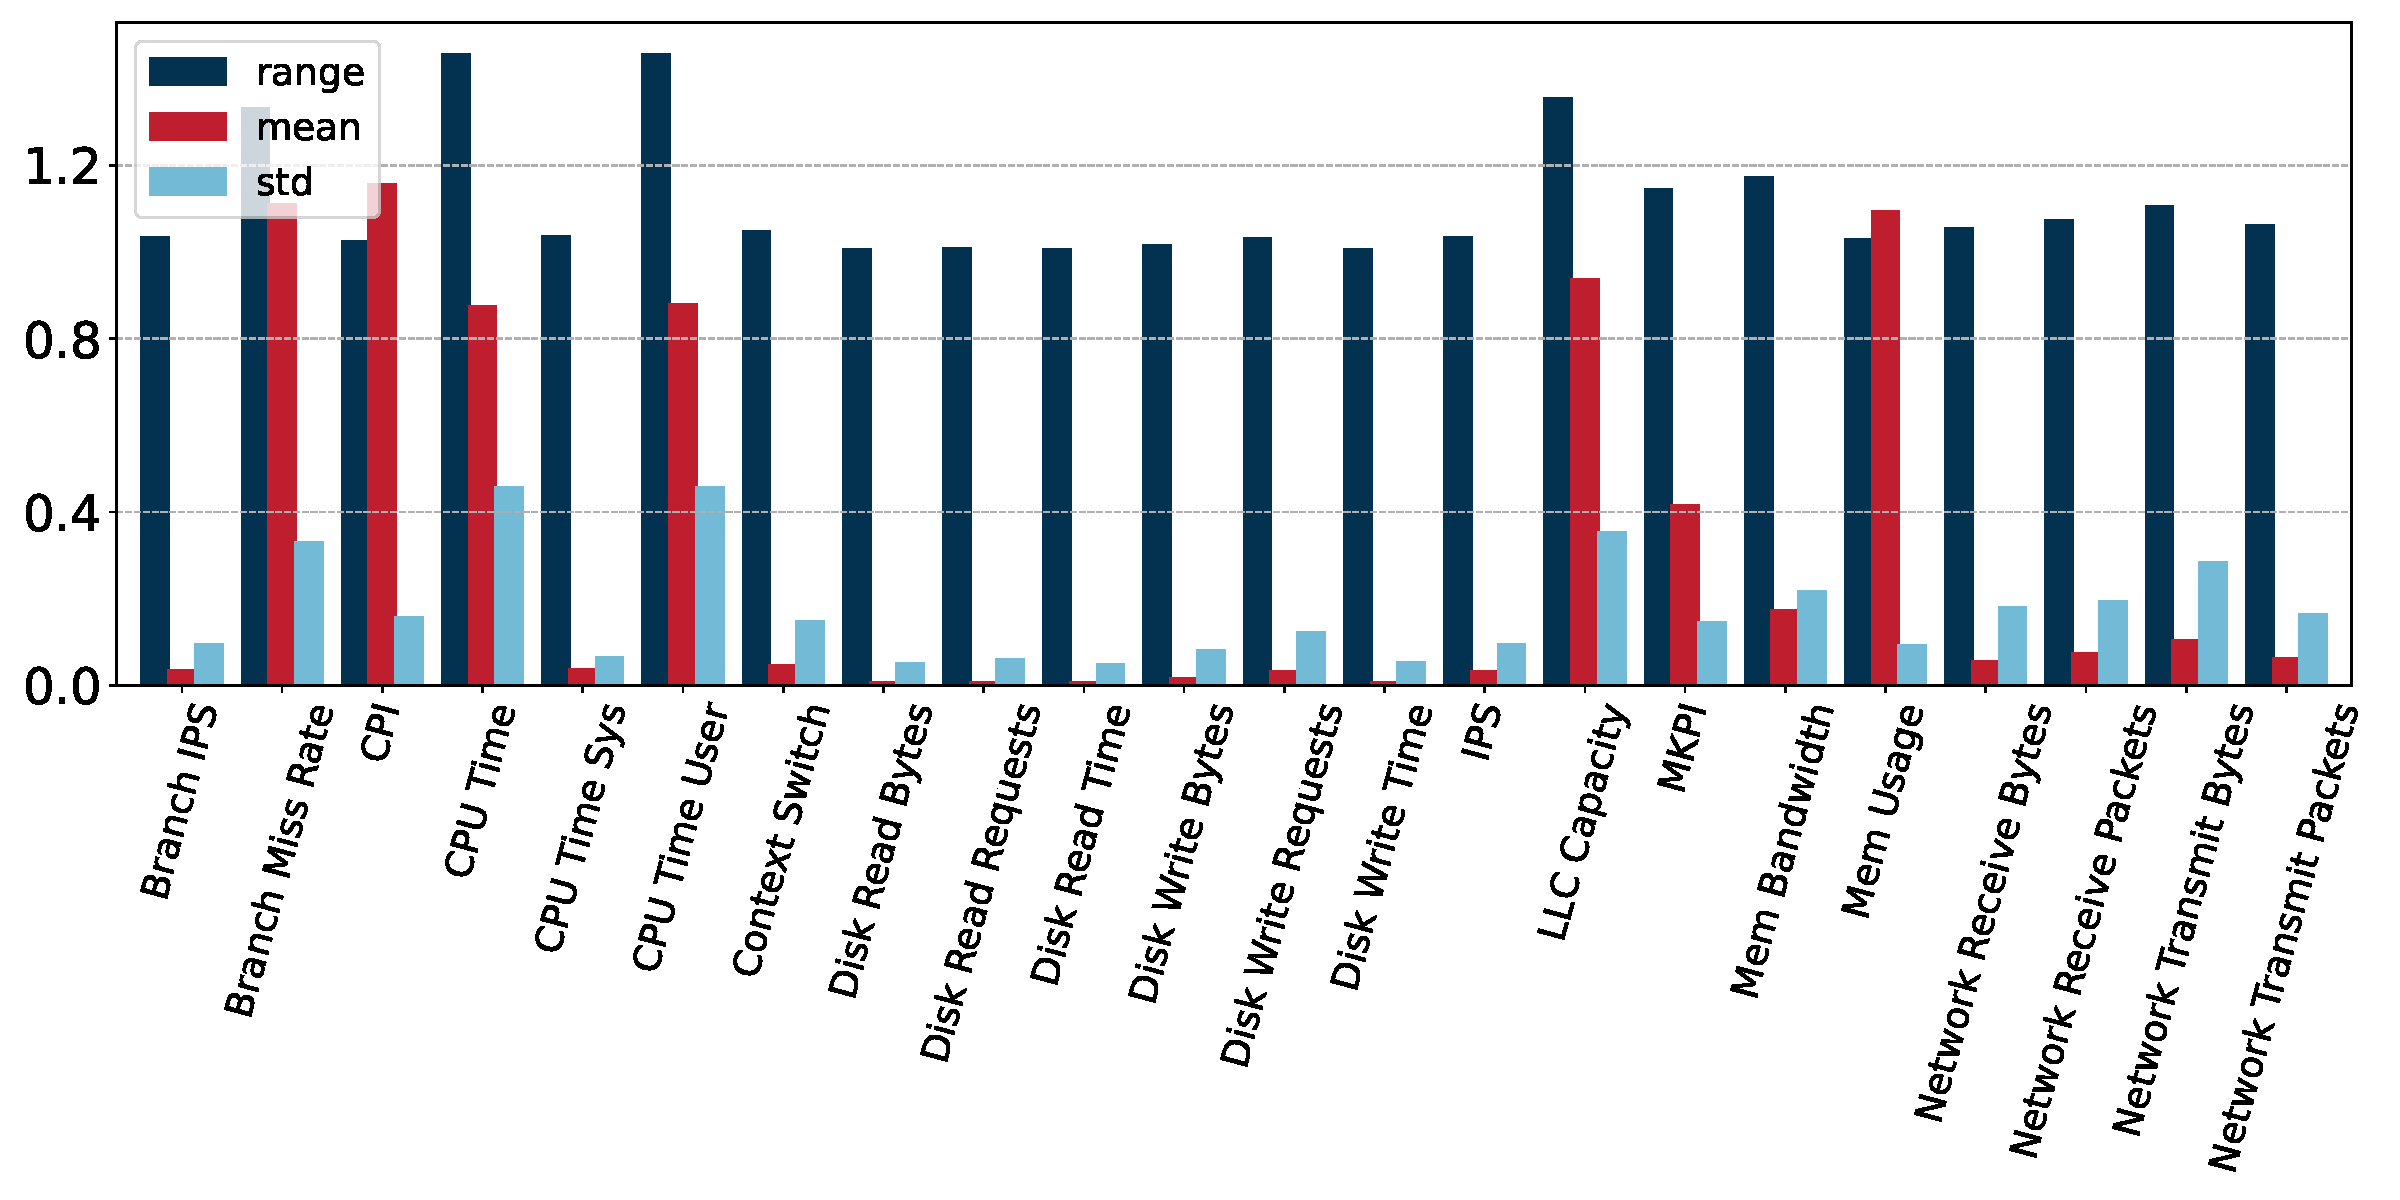
\includegraphics[width=\textwidth]{profile_elasticsearch}
      \caption{Elasticsearch资源使用}
      \label{fig:profile_elasticsearch}
    \end{subfigure}
    \begin{subfigure}[b]{0.85\textwidth}
        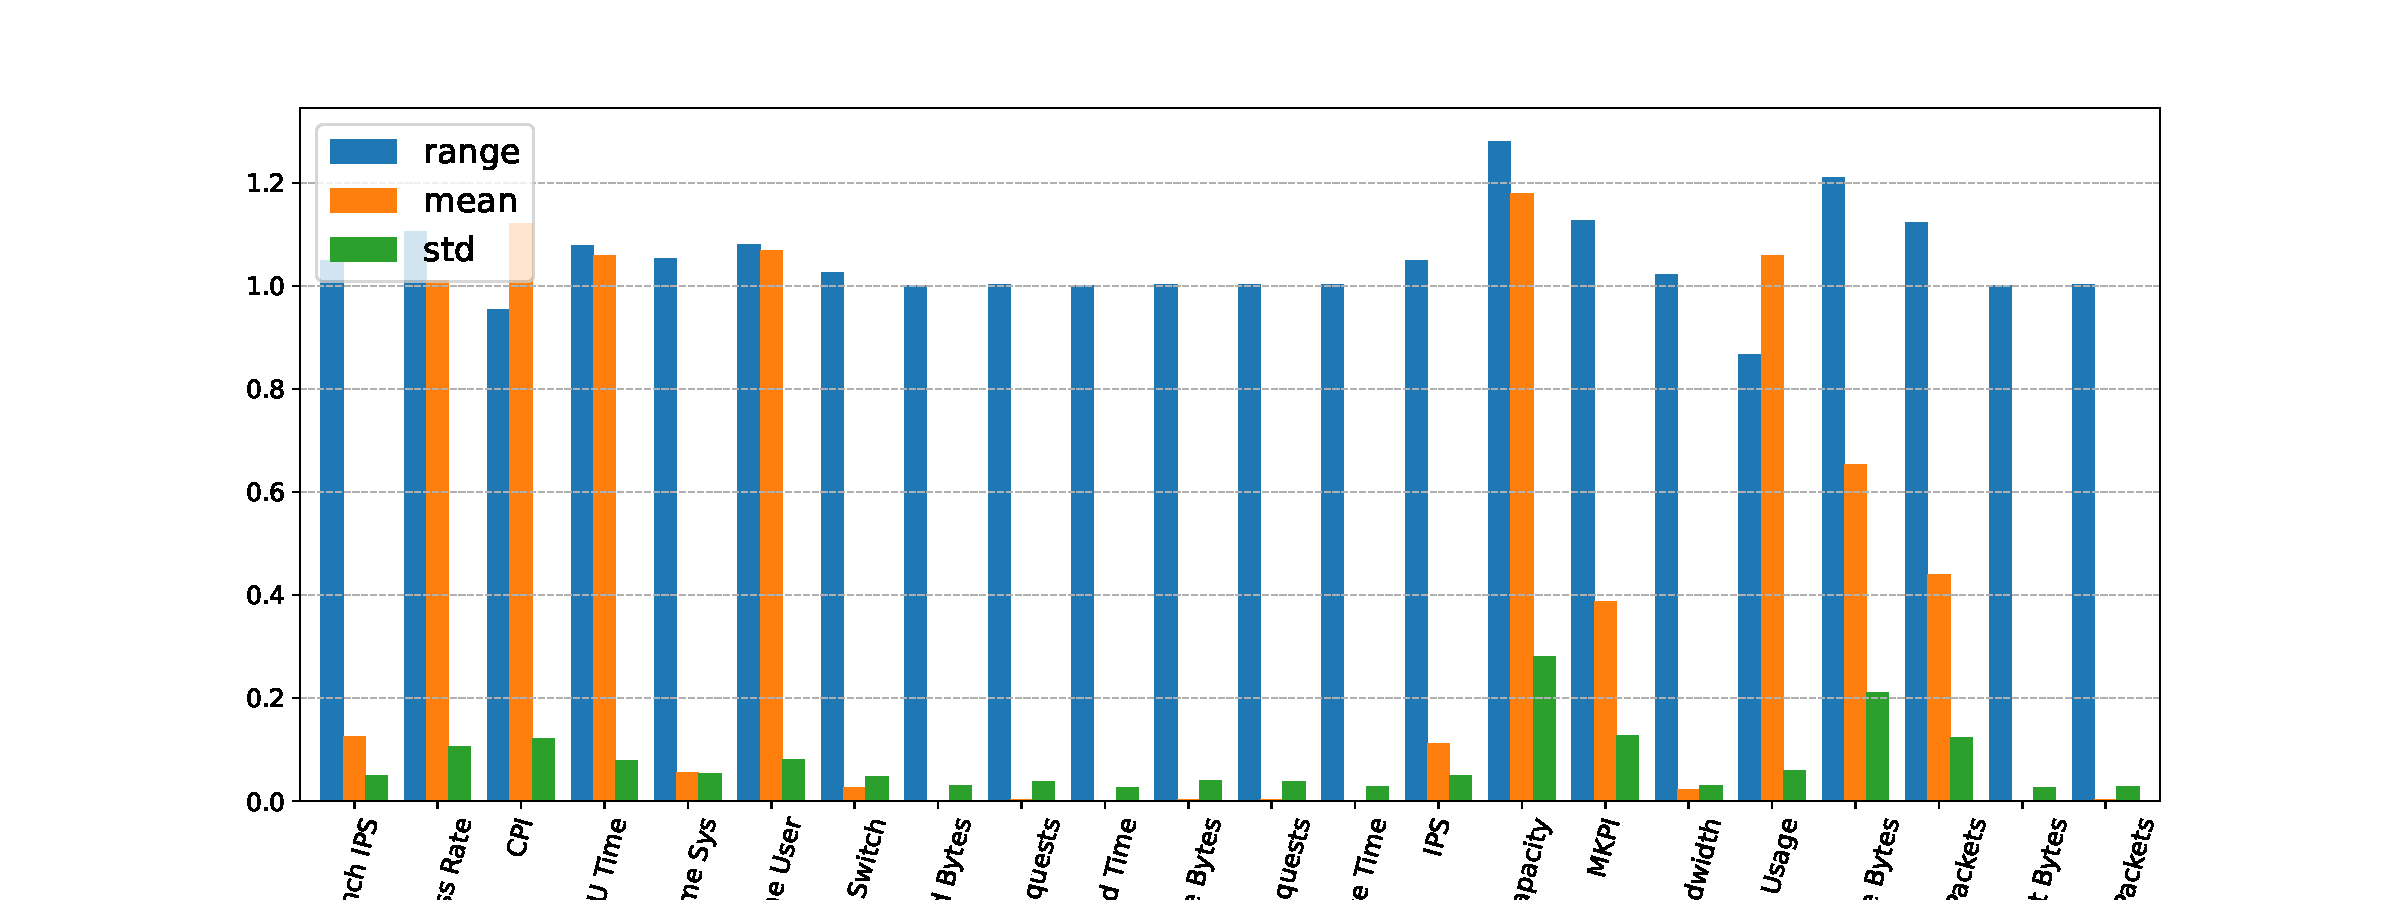
\includegraphics[width=\textwidth]{profile_render}
        \caption{Render资源使用}
        \label{fig:profile_render}
    \end{subfigure}
\bicaption{\quad Elasticsearch与Render资源使用情况}{\quad Resource Usage of Elasticsearch and Render}
\label{fig:resource_affinity_2}
\end{figure}
    
    \item \textbf{I/O资源}:在I/O资源上,不同应用的使用需求差异同样十分大。其中Elasticsearch、Kafka和Mysql由于涉及到存储内容的持久化,因此会大量地使用I/O资源。而类似Redis等应用,虽然存在数据持久化的配置,但实际运行中持久化频率较低,因此通常只会有周期性的少量I/O资源占用。
\end{enumerate}

\section{性能劣化实验设计与分析}

\subsection{干扰实验设计}

% 干扰应用
% - 干扰有效性
% - 噪声控制

性能劣化实验通过增加目标应用与干扰应用的混部场景,分析应用对于不同干扰类型的敏感程度。在干扰应用的选择上,使用stress-ng来产生不同类型的干扰。stress-ng是Linux系统中常用的压力测试工具,能够模拟各种资源的压力场景,而实验中则利用其模拟各种压力场景的特性来制造干扰,并观测目标应用的性能劣化情况。stress-ng提供了丰富的配置参数,本课题选用如表~\ref{tab:arg_list}所示的参数配置,来制造CPU、Cache、内存、IO、Network上的干扰。

\begin{table}[H]
    \centering
    \bicaption{\quad stress\_ng 实验参数列表}{\quad stress\_ng args list}% caption
    \footnotesize% fontsize
    \setlength{\tabcolsep}{20pt}% column separation
    \renewcommand{\arraystretch}{1.25}% ro w space 
    \label{tab:arg_list}
    \begin{tabular}{llc}
        \hline
        %\multicolumn{num_of_cols_to_merge}{alignment}{contents} \\
        %\cline{i-j}% partial hline from column i to column j
        子系统 & 参数 & 说明\\
        \hline
        CPU	    & --cpu & 循环执行sqrt(rand())的线程数量\\
	            & --cpu-load & 线程负载的比率\\
        Cache	& --cache & cache抖动线程数量\\
	            & --cache-level	&测试指定等级的Cache\\
	            & --icache	&指令cache抖动的线程数量\\
        IO	    & --io	&循环执行sync()的线程数量\\
	            & --iomix	&执行混合I/O操作的线程数量\\
	            & --hdd	&循环执行write()/unlink()的线程数量\\
	            & --seek	&执行随机seek I/O的线程数量\\
        Memory	& --vm	&循环执行匿名mmap的线程数量\\
	            & --vm-bytes	&执行vm操作的buffer大小\\
	            & --memrate	&执行read/writes的线程数量\\
	            & --memrate-bytes	&执行内存操作的buffer大小\\
	            & --malloc	&执行malloc/realloc/free的线程数量\\
	            & --memcpy	&执行memory copy的线程数量\\
        Network	& --sock	&执行Socket I/O的线程数量\\
	            & --epoll	&执行epoll处理的线程数量\\
        \hline
    \end{tabular}
\end{table}

正式干扰实验之前,首先需要验证干扰的效果。测试实验使用一个4 CPU 8G Memory虚拟机,并在其中按照上述配置运行stress-ng干扰应用。干扰强度的定义与配置的stress-ng线程相关,对于CPU干扰,采用线性的干扰强度,即干扰强度正比于CPU负载,而对于其他干扰则使用指数映射,即干扰强度与线程数量呈指数关系,以便于快速探测干扰峰值。具体实验的结果从可观测性系统中获取,每种干扰选择一个表征指标用以说明,具体结果如图~\ref{fig:interference}所示:

\begin{itemize}
    \item \textbf{CPU干扰}:使用进程CPU使用率作为表征指标,恰好占满所有CPU时的参数配置作为CPU干扰强度100\%的定义。实验干扰效果如图~\ref{fig:cpu_interference}所示,随CPU干扰强度的不断提升,干扰应用能够完全占用CPU资源。CPU干扰强度与干扰效果几乎呈线性关系,但在强度较低时存在波动。
    
    \item \textbf{Cache干扰}:使用Resctrl统计进程的LLC Usage作为表征指标,恰好占满进程所属Numa的LLC时的参数配置作为Cache干扰强度100\%的定义。实验中干扰效果如图~\ref{fig:cache_interference}所示,随Cache干扰强度的不断上升,干扰应用逐渐能够占用全部的LLC。而在前段部分,Cache占用上升较快,而在后段上升由于Cache总量有限,于是上升速度变慢。

    \item \textbf{IO干扰}:使用IO Throuphput Bytes作为表征指标,并将虚拟机IO接近完全占用时的参数配置作为IO干扰100\%的定义。实验干扰效果如图~\ref{fig:io_interference}所示,在前段,随干扰强度的上升,干扰应用占用越来越多的IO带宽,但在后段,由于IO线程的增加,在有限的CPU资源下这些IO线程彼此之间出现相互竞争,导致IO吞吐量上升速度变慢,而在实验过程中发现,更高的配置不仅无法使得IO占用上升,反而由于干扰应用内的较大竞争,导致IO吞吐下降,因此IO干扰配置选用接近最大吞吐时的配置。

\begin{figure}[H]
  \centering
  \begin{subfigure}[b]{0.32\textwidth}
    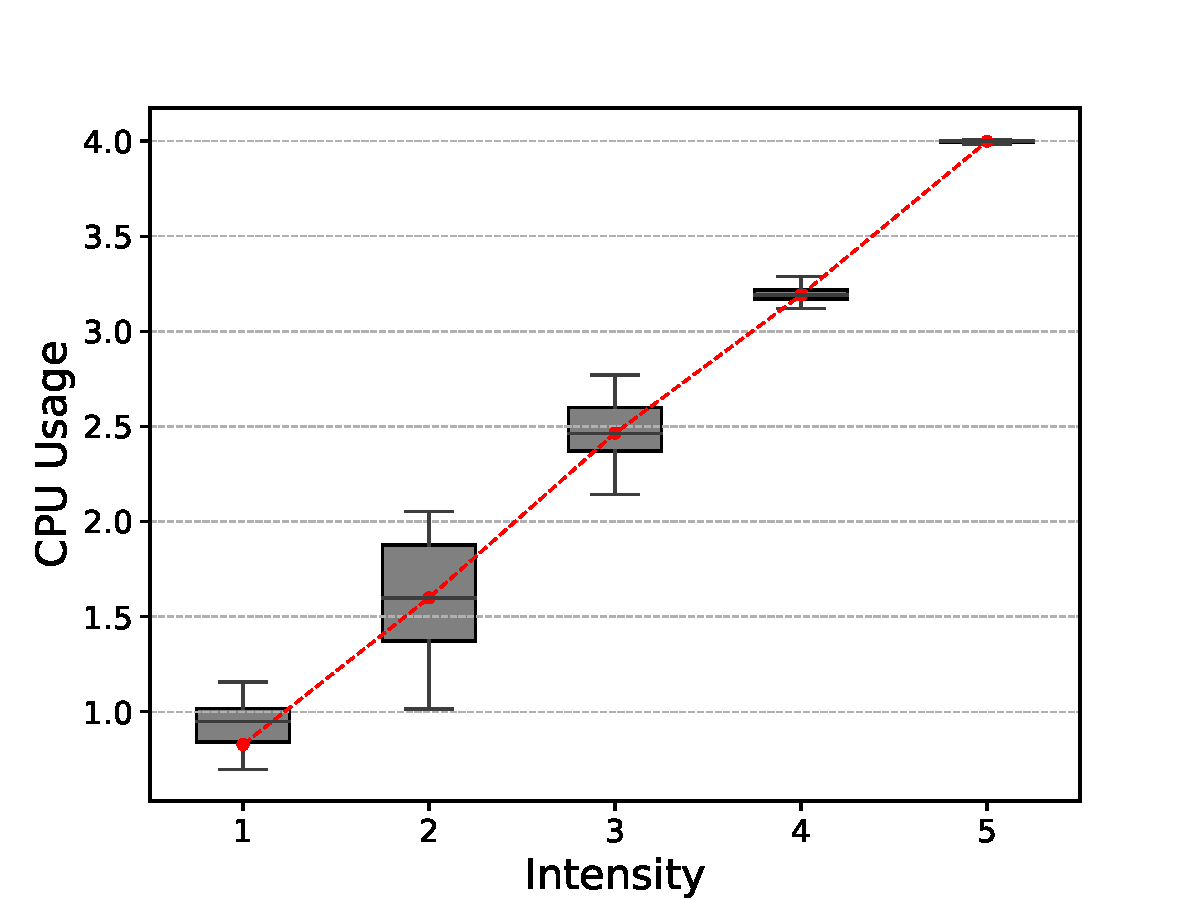
\includegraphics[width=\textwidth]{cpu_interference}
    \caption{cpu干扰效果}
    \label{fig:cpu_interference}
  \end{subfigure}
  \begin{subfigure}[b]{0.32\textwidth}
    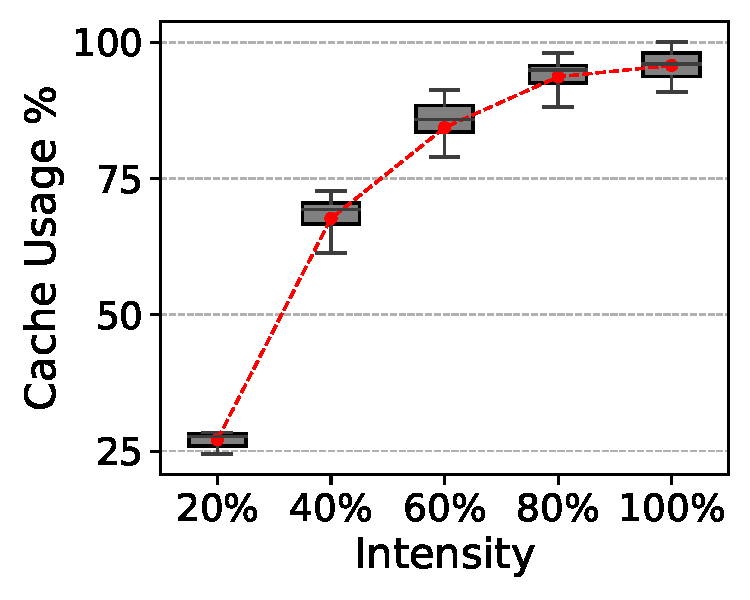
\includegraphics[width=\textwidth]{cache_interference}
    \caption{cache干扰效果}
    \label{fig:cache_interference}
  \end{subfigure}
  \begin{subfigure}[b]{0.32\textwidth}
    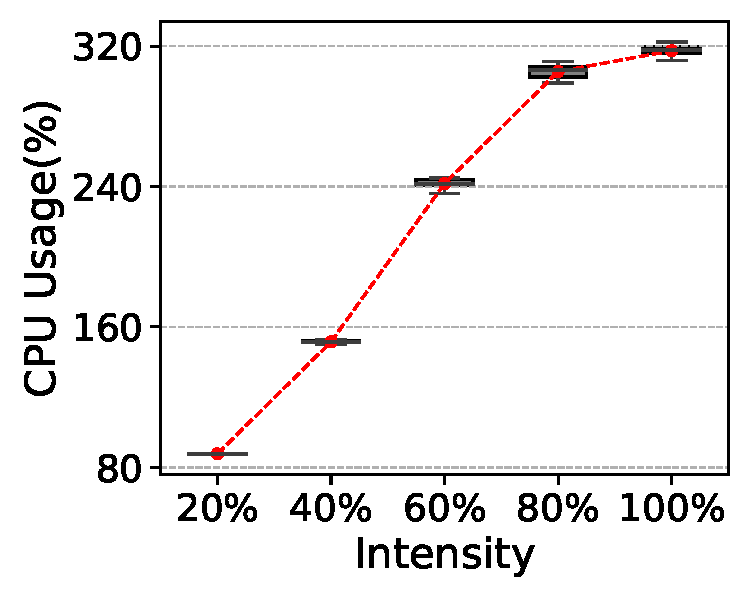
\includegraphics[width=\textwidth]{io_interference}
    \caption{io干扰效果}
    \label{fig:io_interference}
  \end{subfigure}
  \begin{subfigure}[b]{0.32\textwidth}
    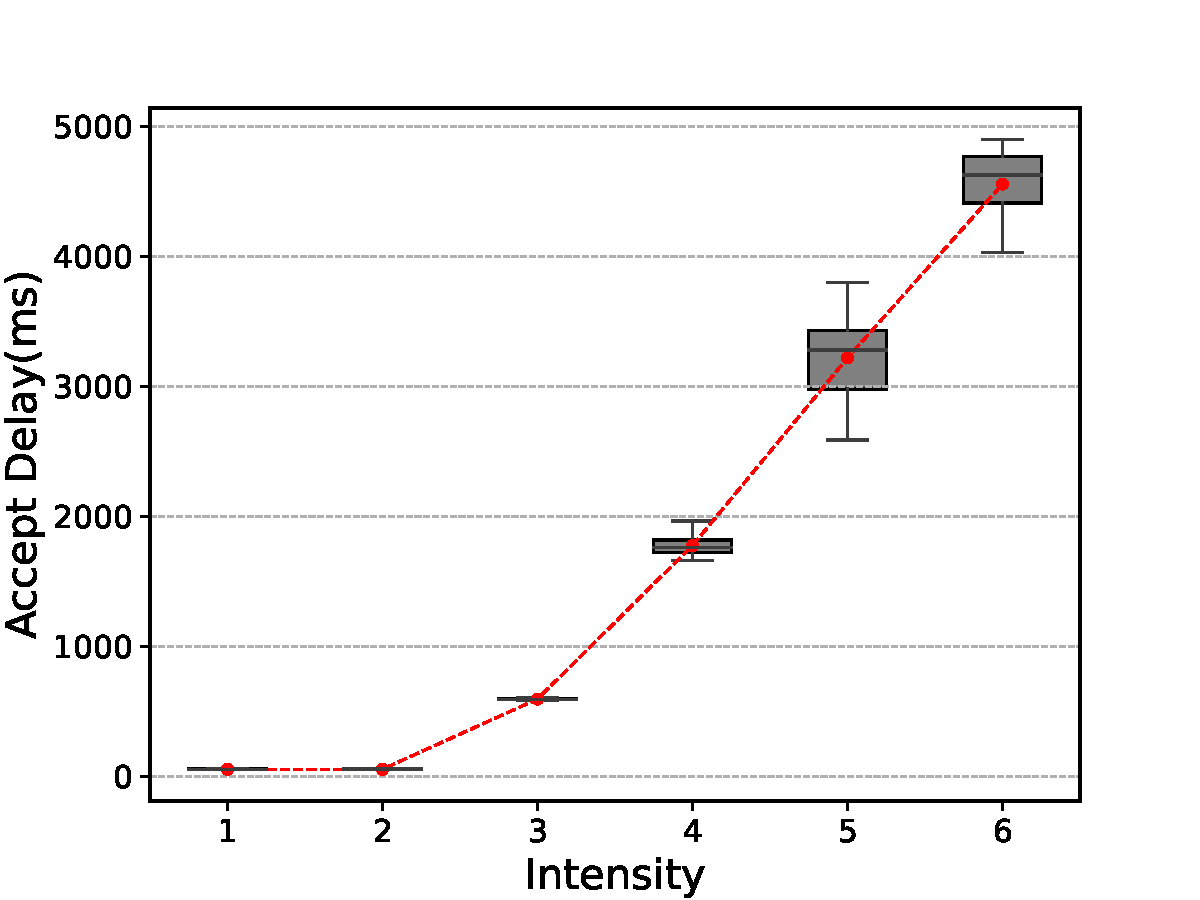
\includegraphics[width=\textwidth]{net_interference}
    \caption{net干扰效果}
    \label{fig:net_interference}
  \end{subfigure}
  \begin{subfigure}[b]{0.32\textwidth}
    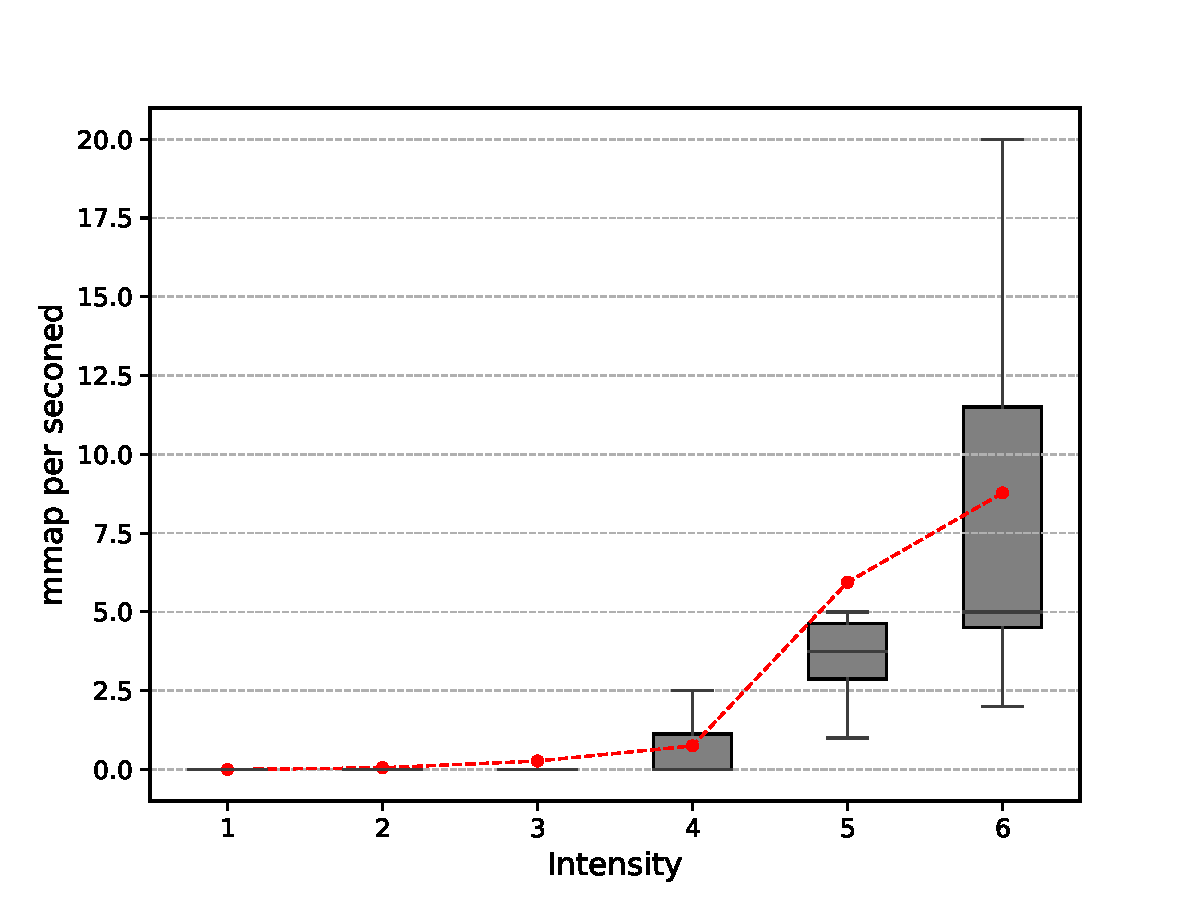
\includegraphics[width=\textwidth]{vm_interference}
    \caption{内存干扰效果}
    \label{fig:vm_interference}
  \end{subfigure}
  \bicaption{\quad 干扰效果分析}{\quad Interference Effects Analysis}
  \label{fig:interference}
\end{figure}

    \item \textbf{Net干扰}:使用网络子系统中的Accept系统调用延时作为表征指标。Linux中,Accept系统调用通常由Server类应用调用,用来与Client建立连接吗,而Accept系统调用执行速度变慢通常意味着连接排队延迟与客户端超时,由于延时并没有最大值,因此实验中选择延时上升速度加快的干扰配置作为100\%的定义。实验干扰效果如图~\ref{fig:net_interference}所示,可见随干扰强度的不断上升,Accept系统调用的延迟逐渐变大。
    
    \item \textbf{Memory干扰}:使用每秒的mmap系统调用次数作为表征指标。stress-ng通过频繁地调用mmap来产生内存干扰,而频繁的内存分配操作会对内存子系统施加干扰,实验中选择mmap频率波动较大的干扰配置作为Memory干扰100\%的定义。实验干扰效果如图~\ref{fig:vm_interference}所示,随干扰强度的上升,每秒的mmap系统调用数量也在不断上升,并在干扰强度最大时出现较大的波动。
\end{itemize}

考虑到干扰效果评测结果中,Net干扰实际上使用的是本地回环网络,因此并不能实质性地在网络流量上产生干扰,导致类似于CPU或Cache干扰,因此在后续的
没有采用Net干扰项作为测试项,而是根据典型应用的类型,如是否是网络应用来判断应用的网络敏感性。

\subsection{典型应用资源敏感度分析}

资源敏感度主要分析典型应用与不同配置下的干扰进行混部后的性能劣化情况,其中应用性能使用竖亥Benchmark提供的白盒指标进行评价。白盒指标中既有经过加权计算后的统一评分,也有对于每个应用单独的评价指标,在性能劣化中,主要选择劣化程度与干扰程度较为相关的指标进行分析。

\begin{figure}[H]
    \centering
    \begin{subfigure}[b]{0.32\textwidth}
        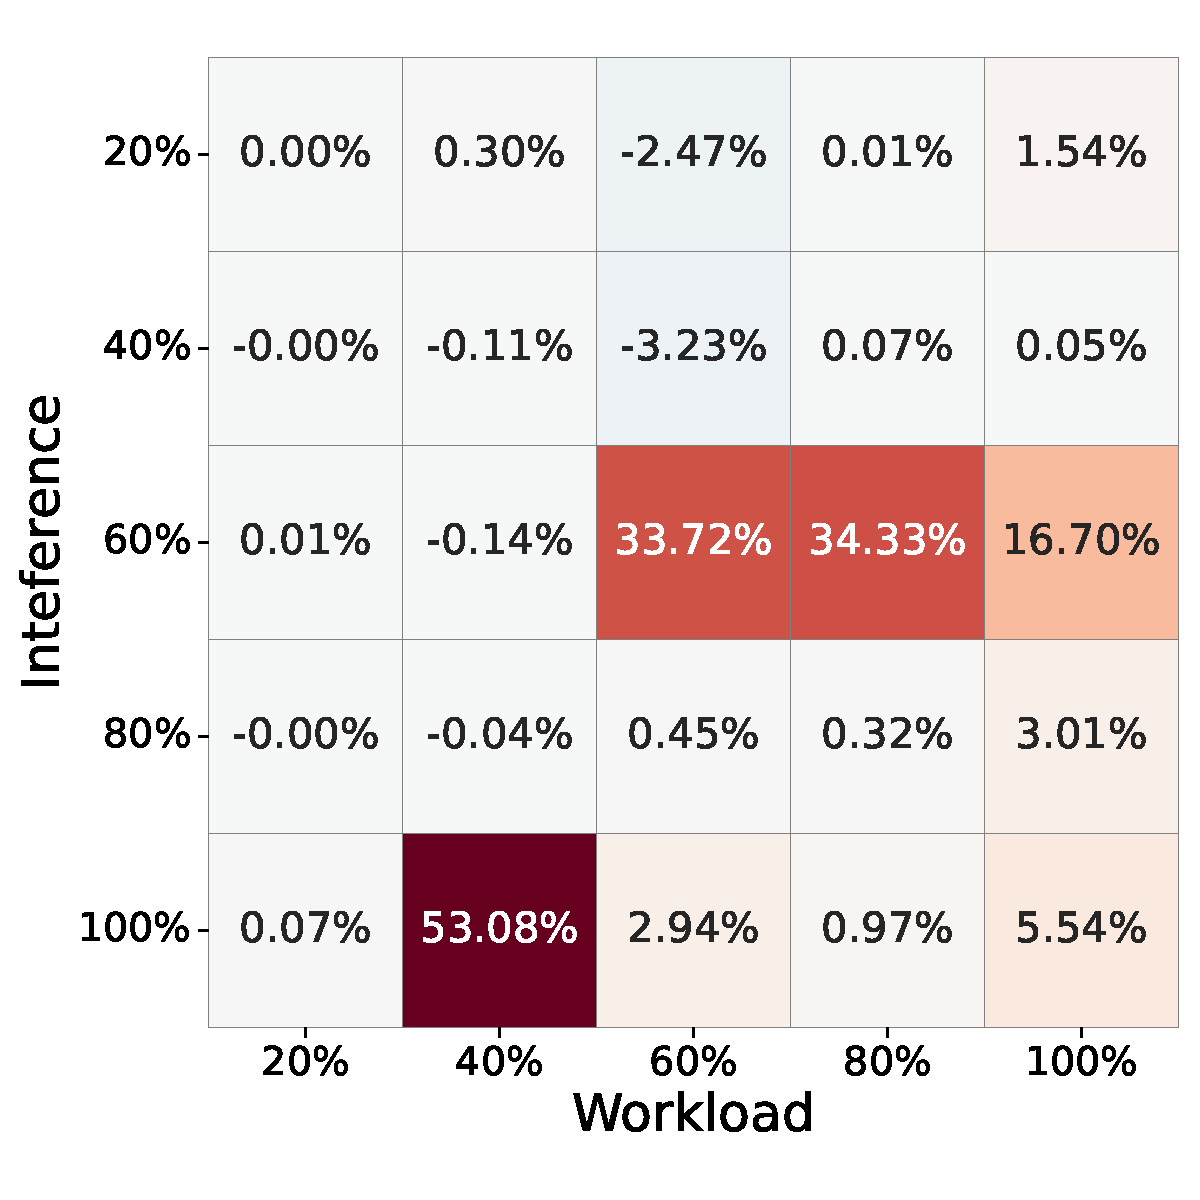
\includegraphics[width=\textwidth]{interfer_cpu}
        \caption{CPU干扰下的性能劣化}
        \label{fig:interfer_cpu}
    \end{subfigure}
    \begin{subfigure}[b]{0.32\textwidth}
      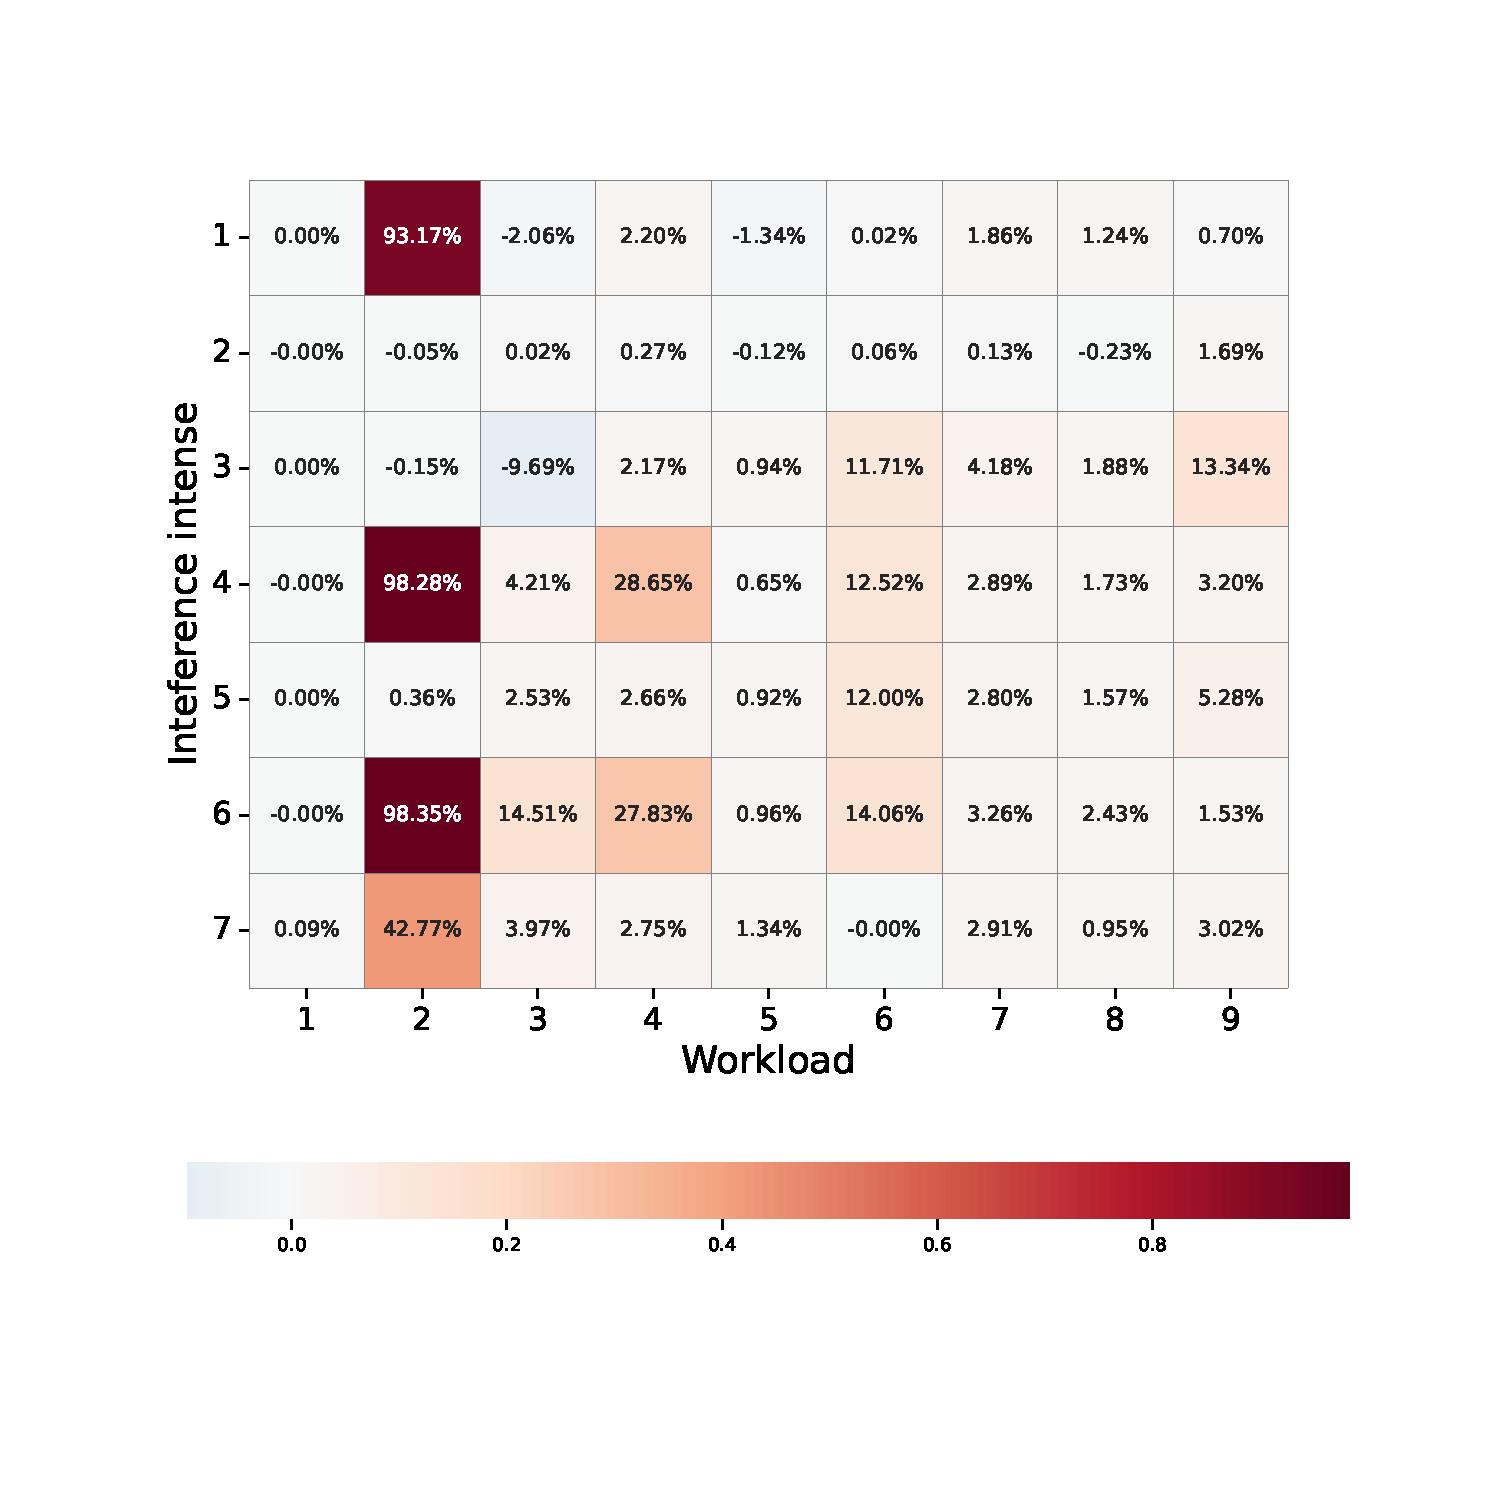
\includegraphics[width=\textwidth]{interfer_cache}
      \caption{Cache干扰下的性能劣化}
      \label{fig:interfer_cache}
    \end{subfigure}
    \begin{subfigure}[b]{0.32\textwidth}
        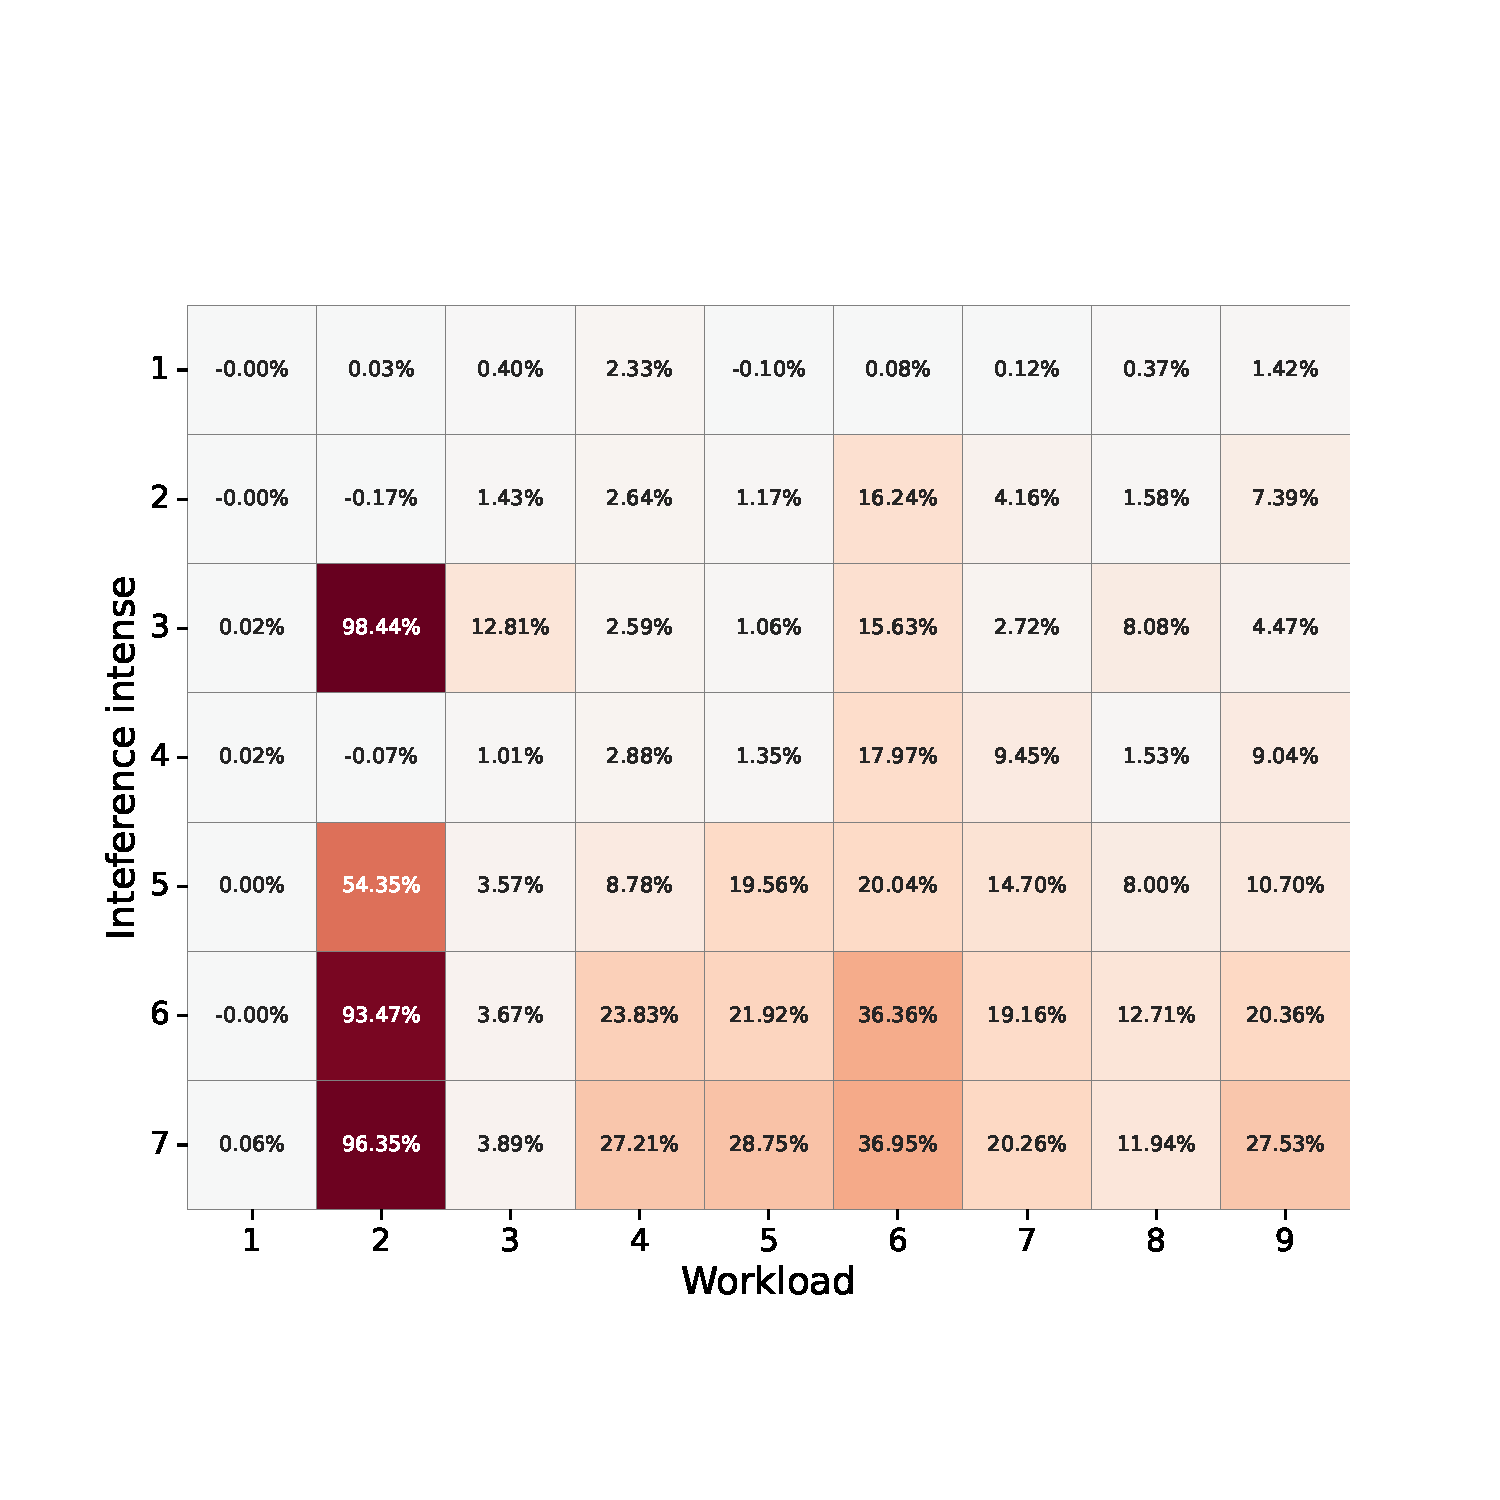
\includegraphics[width=\textwidth]{interfer_mem}
        \caption{Memory干扰下的性能劣化}
        \label{fig:interfer_mem}
    \end{subfigure}
    \begin{subfigure}[b]{0.32\textwidth}
        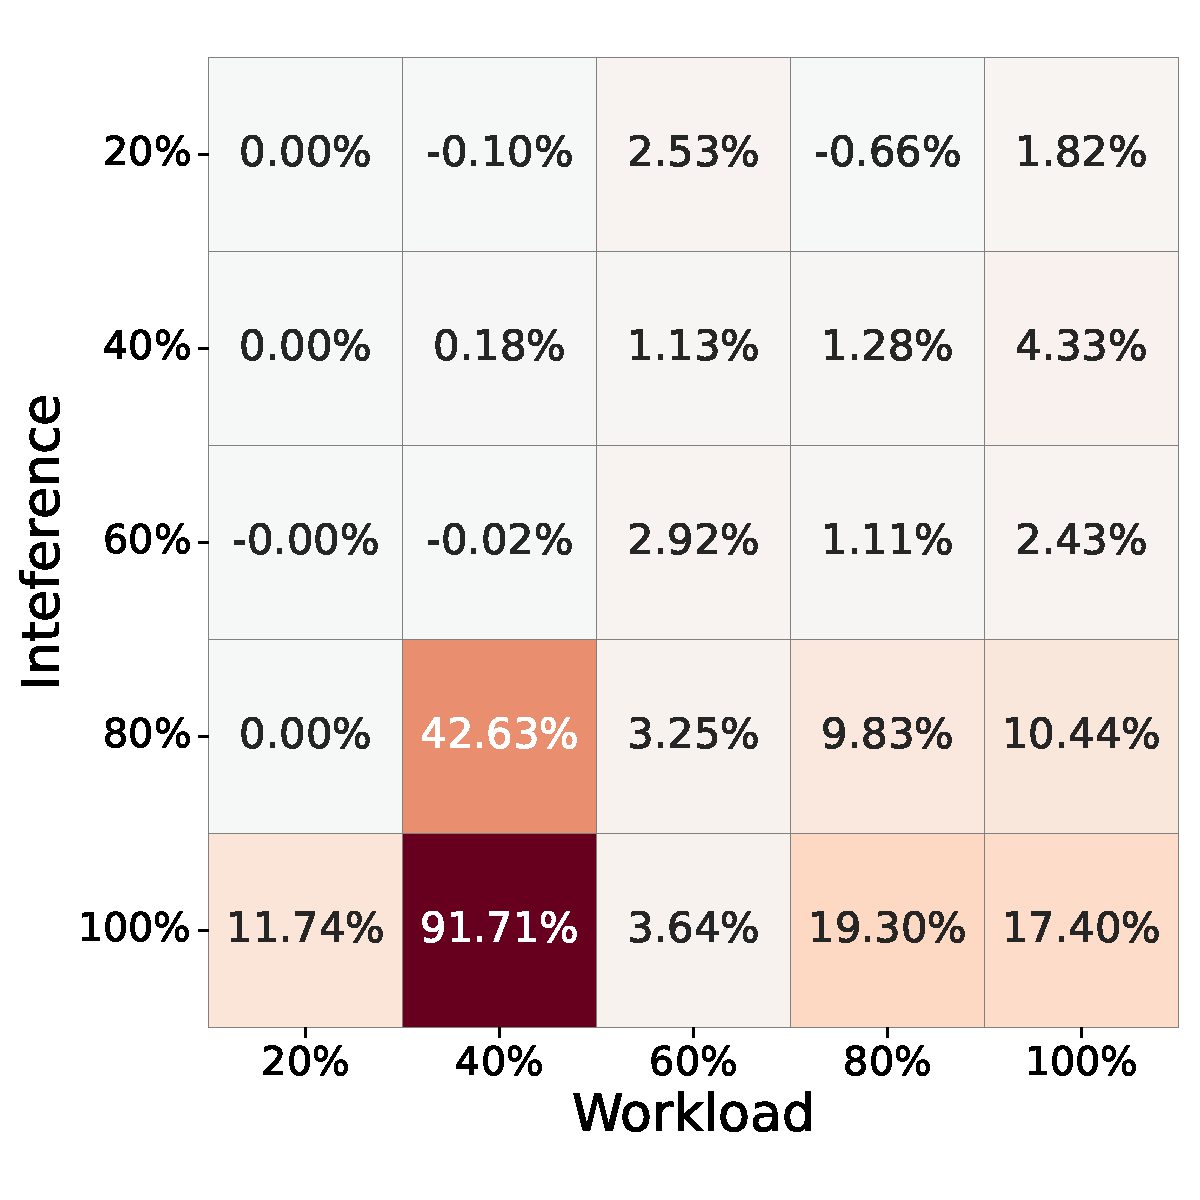
\includegraphics[width=\textwidth]{interfer_net}
        \caption{Net干扰下的性能劣化}
        \label{fig:interfer_net}
    \end{subfigure}
    \begin{subfigure}[b]{0.32\textwidth}
        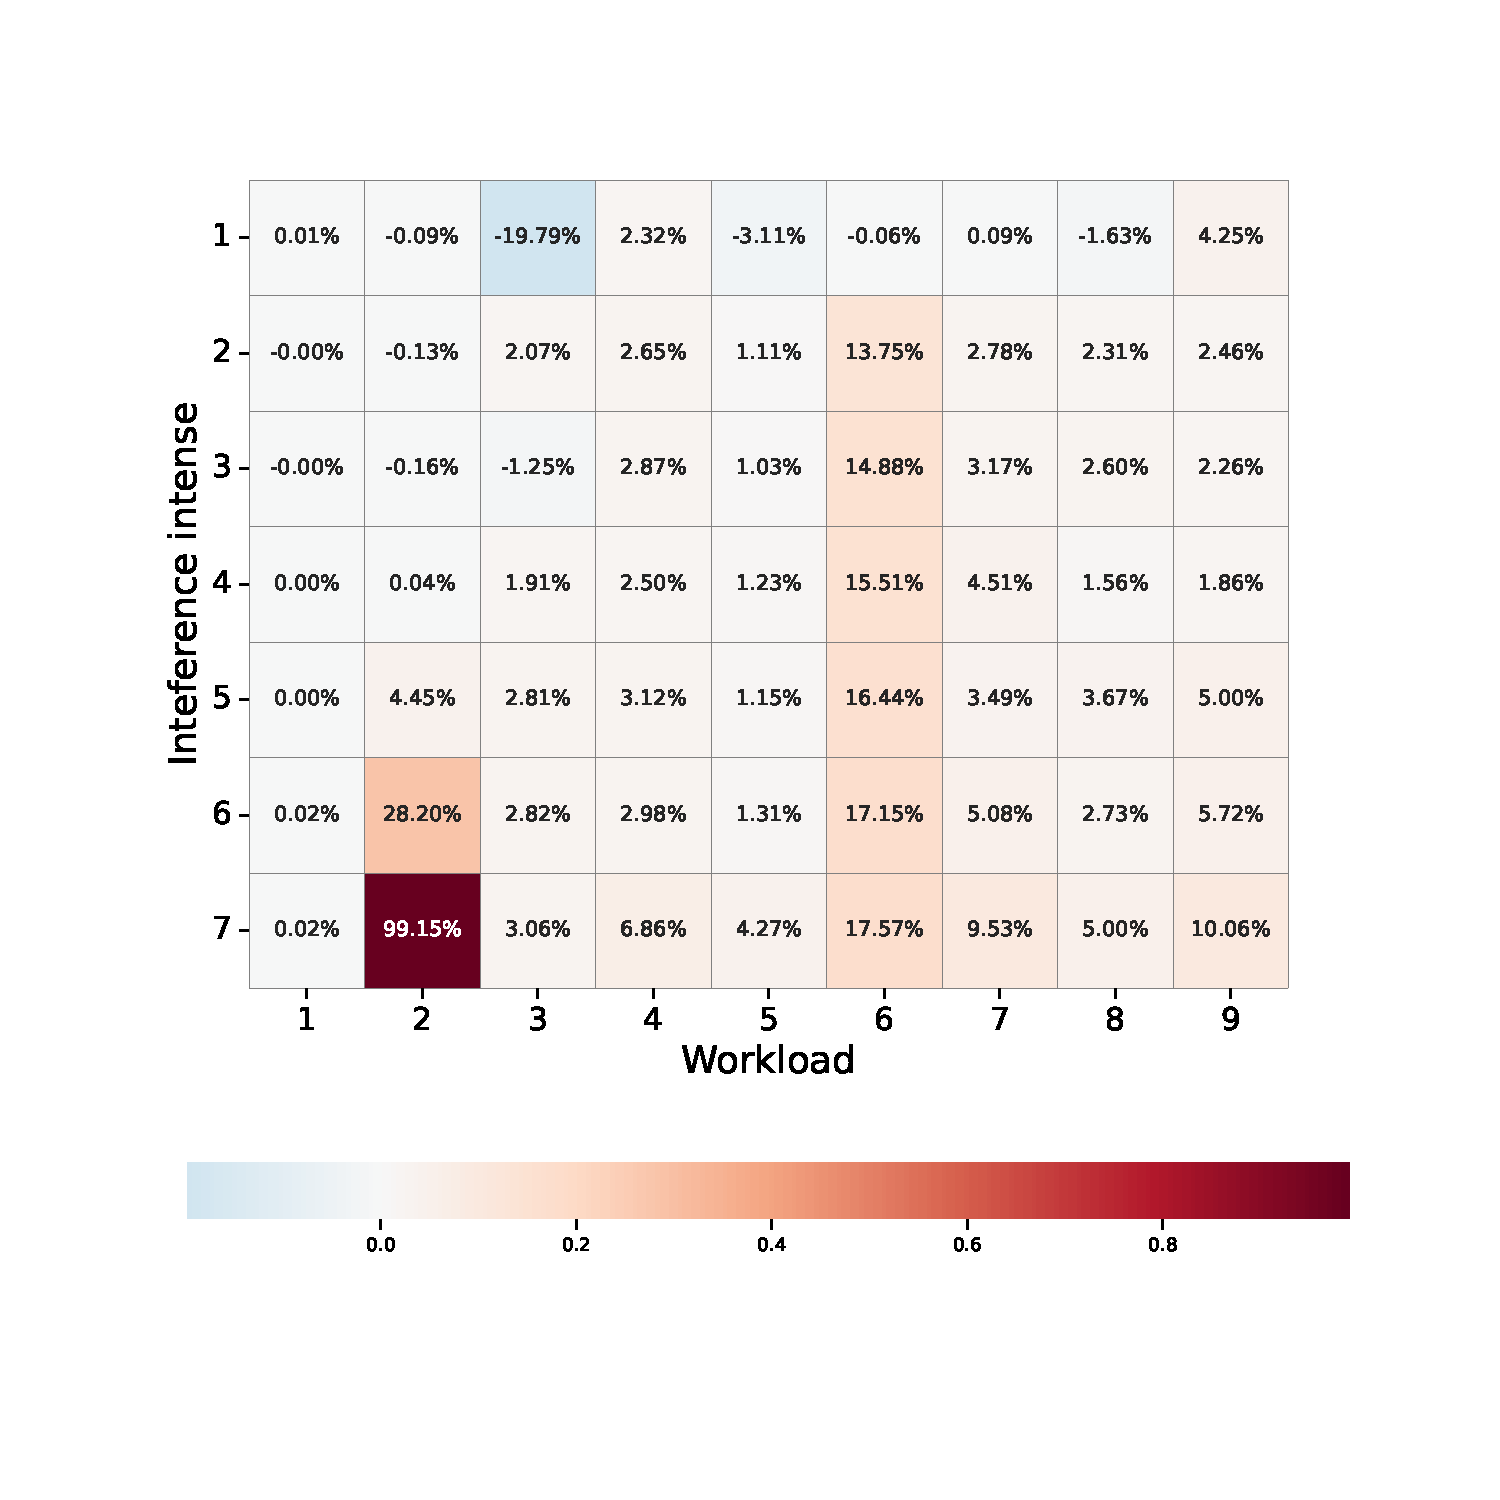
\includegraphics[width=\textwidth]{interfer_io}
        \caption{IO干扰下的性能劣化}
        \label{fig:interfer_io}
    \end{subfigure}

\bicaption{\quad Redis干扰敏感度}{\quad Redis interference sensitivity}
\label{fig:redis_interf_sensitivity}
\end{figure}

以Redis为例,使用redis操作延迟作为性能评价指标,计算有无干扰下的指标变化百分比用于描述劣化程度,综合不同干扰及不同负载下的实验结果如图~\ref{fig:redis_interf_sensitivity}所示。

结合其他应用的资源敏感性分析,可从资源的角度对典型应用进行初步划分,主要为如下3类:

\begin{enumerate}
    \item \textbf{单纯CPU敏感型}:此类应用对于CPU干扰最为敏感,而受其他干扰影响的程度则明显更低。如Memcached,其在受到CPU资源干扰后产生了近50\%的性能劣化,而对于在其他干扰下的劣化程度则在10\%内,同样的情况也在Kafka的实验数据中出现。
    \item \textbf{CPU与Cache敏感型}:此类应用同时受CPU与Cache干扰明显,且通常对CPU干扰更加敏感。如Redis,与Memcached类似,对CPU干扰十分敏感,而同时由于Redis没有开启多线程支持,因此在Cache资源上的竞争能力弱于Memcached,从而更容易受到Cache干扰的影响。Elasticsearch情况则更为复杂,竖亥Benchmark中提供了不同的白盒指标来表征Elasticsearch的性能,主要分为吞吐量与延迟,以吞吐量作为标准,则Elasticsearch符合CPU敏感型,而以延迟作为标准,则Elasticsearch则更倾向于CPU和Cache敏感型,这种现象在其他典型应用中也有出现,而对于Elasticsearch,其使用场景中更注重吞吐量,因此在本文中将其归类为CPU与Cache敏感型。
    \item \textbf{资源不敏感型}:此类应用对于所有干扰的敏感度都偏低。实验中Render在各个干扰下都没有出现较为明显的劣化,这主要有两个原因。一方面,在性能指标上,Render应用使用了完成时间作为性能评价指标,而与其他应用的性能指标不同,完成时间这一指标更偏向于整个运行过程的总体性能述而不是单一处理过程的性能,一些突发的性能劣化不会体现在这一指标上,另一方面,内核调度机制上在未作限制时倾向于公平地分配时间,因此干扰程序会因调度的影响向Render出让CPU时间,而当CPU资源总和足够满足Render使用时,性能指标就不会出现较大变化。
\end{enumerate}

\section{本章小结}

本章主要论述了对云场景典型应用进行画像分析的过程,围绕三个问题展开。首先,在软件环境上,结合与云厂商的合作经验确定了以虚拟机作为应用运行时的典型云场景,随后通过对数据中心软件栈的分析,选取了7种典型应用作为画像分析的对象,涵盖了传统数据库、键值存储、消息中间件、媒体处理等领域。

随后,为解决引入虚拟化所带来的黑盒监测难题,基于Prometheus生态设计实现了一套面向虚拟机的可观测性系统,从Host、Hypervisor到Guest等多个维度以虚拟机为粒度采集丰富的指标数据。本文主要设计实现了Libvirt Exporter、KVM Exporter、Resctrl Exporter以及Kernel Exporter四种采集组件。其中创新性地引入eBPF技术,在应用与内核交互的关键路径,内核与设备交互的关键路径上进行采样分析,获取更丰富的指标数据。

最后,围绕典型应用的资源使用倾向与资源敏感度展开实验分析。其中首先对干扰应用进行参数搜索,找到制造CPU、Cache、Memory、IO以及Network五种干扰的合适参数,并与典型应用进行混部实验。在资源使用倾向上,分析了典型应用资源使用倾向分类,而在资源敏感度上,总结了得到了典型应用的干扰敏感度评级。